\chapter{Research Avenues}
\label{ch:researchavenues}
% ##################################################################################################################

\hfill \textbf{Authors:} Kai Nagel, Kay W.\ Axhausen, Benjamin Kickhöfer, Andreas Horni

\begin{center} 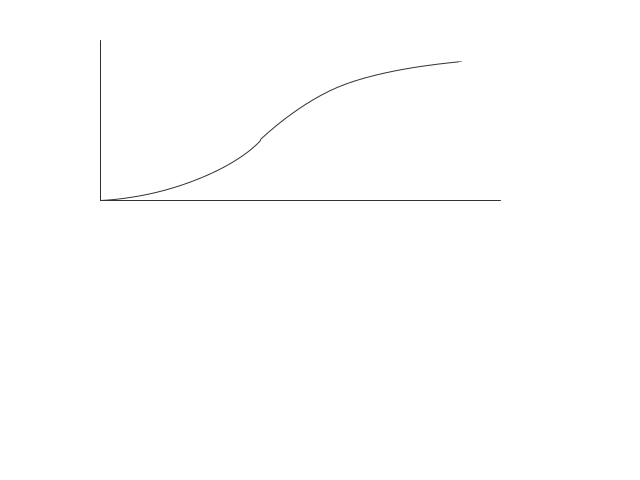
\includegraphics[width=0.4\textwidth, angle=0]{figures/stable-activity-allocations} \end{center}

% ##################################################################################################################
The on-going work and the interest documented in the many scenarios shows 
that the system has not exhausted its possibilities as a platform for research on it and with it. 
This chapter wants to highlight some of them for further discussion and maybe action. 

% ##################################################################################################################
\section{MATSim and Agents}
\label{sec:matsim-and-agents}

%% , and Travel Behavior Research}

% Q-learning: learn utility for each state-action pair
%
% utility learning: learn utility for each state
%
% difference: In the second case, need to have a model about the world.  I.e. need to know which actions lead to which probabilities for the next state.

% 20.2 passive learning in a known environment

% naive: proceed until terminal state, backpropagate utility to all previous states, average over all such utility values ever collected per state

% adaptive dynamic programming: U(i) = R(i) + \sum_j M_{ij} U(j)

% where R(i) is the reward at i and M_{ij} are the transition probas 
% (recall that this is passive learning)

% I don't that that this can be sampled ... needs to solve the equations

% temporal difference (TD) learning: U(i) <-- U(i) + alpha * ( R(i) + U(j) - U(i) ) 

% 20.3 passive learning in an unknown environment

% Since TD never neede M_{ij}, it will still work as before.  Will now also 
% learn M_{ij}, but separately

% 20.4 active learning in an unknown environment

% Now M^a_{ij} (depending on the action)

% U(i) = R(i) + max_a \sum_j M^a_{ij} U(j)

% TD approach same as before

% 20.5 Exploration

% 20.6 Learning an action-value function (Q values, Q-learning)

\subsection{Complex Adaptive Systems}
\label{sec:complex-adaptive-systems}

The core \gls{matsim} architecture---where agents learn utilities for plans---was originally derived from the field of \acrfullpl{cas} \citep[e.g.][]{AxelrodBook,Holland_1992,HraberJonesForrestEcho,PalmerEtAl_PhysicaD_1994}. 
%% %\kwaah{Has this been spelled out somewhere ?} \ah{yes, gls()}
%% \kwaah{Why not Axelrod (1980) or Schelling: ``Schelling, TC 1978. Micromotives and Macrobehavior. Toronto, Canada: George J. McLeod Ltd.'' mit seinem Segregationsmodell} 
%% \ah{m.E. ist dies sein Seggregationspaper: \citet[][]{Schelling_TJMS_1971} (Issue 2), \citet[][]{Sakoda_TJMS_1971} (Issue 1) war aber sowieso vorher  gemäss Prof. Hegselmann.}
%% \kai{Müsste ich nach dem Urlaub machen.  \url{http://en.wikipedia.org/wiki/File:Map-of-complexity-science.jpg} gäbe ansonsten eine (m.E.\ ganz gute) Idee, welche Autoren man zitieren will.}
%
\citet{ArthurBar} addresses a coordination problem, where agents receive a payoff only when less than 60 out of 100 go to an event.  He addresses this by first generating a large number of heuristic predictors for the next round's attendance, such as ``same as in last round'' or ``trend of last four rounds''.  He next gives each agent a randomly selected handful of these strategies, so that agents in general have different sets of predictors.  Then, many rounds of the game are played, where the score of each predictor is updated based on its prediction quality,  
%\kwaah{payoff?} 
%\kai{nein, eigentlich so, wie es da steht: der score ($=$ payoff) wird angepasst basierend auf der Qualität der Vorhersage.  Wenn es unverständlich ist, was können wir dann tun?}
and agents act based on their currently best predictor.  Simulations demonstrate that the approach leads to successful coordination, \ie around 60\,agents show up in every round.
%
That approach in turn builds on work by \cite{PalmerEtAl_PhysicaD_1994}, who simulate a stock market, \citet{Holland_1992}, whose classifier systems have more structure than in Arthur's model but have a similar model of performance learning, or \cite{AxelrodBook}, who investigates adaptive agent in the face of repeated non-cooperative games.  

\citet{ArthurBar} kept each agent's predictors fixed after initialization.  In contrast,
\citet{HraberJonesForrestEcho} simulate an artificial ecosystem, where the individual agent strategies are based on so-called genes, which are adapted over the rounds/iterations by a genetic algorithms \citep{Goldberg_1989}.

\subsection{Artificial Intelligence}
\label{sec:artif-intell}

The focus of \gls{cas} is on many agents, agent interaction, and emergence. \Acrfull{ai} in contrast concentrates on single agents. In \gls{ai} terms, the original \gls{matsim} agents (those that do day-to-day learning) are very simple 
%active 
reinforcement learning agents \citep[][Chapter 21.3]{RusselNorvig2010ArtificialIntelligence}. Since these \gls{matsim} agents have only one state (the initial/nightly state) and each action is simply a plan, the distinction between Q-learning and utility learning \citep[as defined by][]{RusselNorvig2010ArtificialIntelligence} actually collapses, and what remains is the temporal difference 
%\kwaah{lagged} 
%\kwaah{Maybe better, given the difficult interpretation of the the iterations.} 
%\kai{Würde lieber bei ``temporal difference learning'' bleiben, denn das ist der terminus technicus.} 
learning \citep[again as defined by][]{RusselNorvig2010ArtificialIntelligence} scheme for the utility, which translates to the \gls{matsim} situation by updating the score/performance/utility value of each plan every time it is selected.

%% \subsection{Travel Behavior Research}


\subsection{Synthesis}

That is, overall,
%\kai{von wem kommt das st?  warum?  Ich meine schon ``That is'', aber vielleicht ist der Text nicht klar genug?} \ah{kwa}
the original \gls{matsim} system has inherited the focus on large systems, interaction, and emergence as well as the approach to strategy innovation from \gls{cas}, while the score updating rather comes from the field of \gls{ai}.

In consequence, a somewhat obvious path to move on is to include more aspects of modern \gls{ai} into the \gls{matsim} agents.  Examples include:
\begin{itemize}

\item Extend \gls{matsim} to agents that can react 
immediately, rather than having to wait for the next iteration or round.  In transport, this is sometimes called en-route or within-day replanning \citep[e.g.,][]{EmmerinkEtAl_TransResC_1995,balijepalli-2007, Axhausen_Jones_1990}. 
%\kwaah{Add reference to 
%Axhausen, K.W. (1990) A simultaneous simulation of activity chains, in P.M. Jones (ed.) New Approaches in Dynamic and Activity-based Approaches to Travel Analysis, 206-225, Avebury, Aldershot. 
%}
See Chapters~\ref{ch:withinday} and~\ref{ch:dts} as well as Section~\ref{sec:researchavenues-withinday}.

\item Improve the \gls{matsim} agents with respect to choice set generation.  This may include both a better creative capability of the agents to come up with innovative new strategies to handle their virtual lifes as well as considerations of consistency between choice set generation and estimated choice models.  See Sections~\ref{sec:Evolution-of-choice} and~\ref{sec:choicesets}.

\end{itemize}


%% In the meantime, both \gls{ai} and the field of transport simulation \st{have moved on}, \kwaah{switched their focus of interest} \kai{Ist das zwingend?  Ich finde ``have moved on'' eigentlich besser, weil es ja kein ``switch'' ist, sondern eine Fortsetzung. Vielleicht weiß jemand eine Formulierung, die weniger colloquial ist.} increasingly looking at agents that can react \kai{also below, chk}


%% \kai{to do more}

% ##################################################################################################################
\section{Within-Day Replanning and the User Equilibrium}
\label{sec:researchavenues-withinday}

\mnote{definition}

Within-day replanning, \ie the ability of the agents to respond to the immediate context is the standard mode of operation for simulation models. 
%
In the transport domain, note the traffic flow models as an example, where aspects such as acceleration/braking or lane changing are (obviously) computed reactively while the simulation is running, and not before the simulation starts \citep[e.g.][]{Wiedemann_PhDThesis_1974}.
%
Many traveller-oriented or agent-based models of travel demand adopt the same approach, \cf ORIENT \citep[][]{Sparmann_TechRep_1980}, ORIENT/RV \citep{AxhausenHerz_JTE_1989}, MobiTOPP \citep[][]{SchnittgerZumkeller_ETC_2004}.
%
For many aspects of \acrfull{its} systems, within-day replanning is indispensable \citep[e.g.][]{hall-1993,EmmerinkEtAl_TransResC_1995,Dobler_PhDThesis_2013}.
%
%% and all the work on intelligent transport system 
%% \kwaah{do we have more?})
None of these systems aim for equilibrium in the sense adopted by \gls{matsim} carried forward from \gls{transims} and ultimately inherited from static assignment.

\mnote{equilibrium with conditional strategies not same as equilibrium with fixed plans}

One may argue that, if supplied with a learning approach, these within-day models should approach equilibrium after many iterations, as the agents with a suitable memory structure would avoid plans which make them worse off. 
%
This memory, which would need to be agent-specific and covering the very large set of choice options, makes the approach costly to implement.
%
Importantly, the solutions may be different: When faced with a stochastic environment, an agent that is able to react within-day can be better off than an agent that follows a pre-computed plan. This is important: Finding a plan with the highest expected score is not the same as finding a conditional strategy with the highest expected score.  

Still, there are context where this immediate response ability can be used within \gls{matsim} to explore the choice set more effectively, especially if the choice alternatives are limited in number and in geographic reach. 
\citet[][]{WaraichEtAl_TechRep_IVT_2013_2}
%Waraich et al. (200x) 
%\kwaah{What is the best reference here?} 
%\ah{afaik, this approach never come beyond a conceptual paper.}
proposes a 
%localized within-day, actually 
within-trip replanning to find the best parking space around a destination.
This localized search reduces the need for full iterations considerably and allows to add behavioral detail at this point, here the type of parking, walking distance to final destination, and parking fee trade-off. 
%In the same spirit, Horni (2015) \kwaah{Gibt es da schon etwas?} \ah{not yet} employs the same approach to address crossing of signalized intersections. 

While within-day replanning can be used as described above within the framework equilibrium search, it can also be added to open up the \gls{matsim} framework to context where such an equilibrium is inappropriate. 
%
\citet[][]{Dobler_PhDThesis_2013} uses the \gls{matsim} calculated equilibrium as the starting point for his model of evacuations and the behavior of the evacuees. 
He also documents that his approach finds a set of executed plans which is close to the \gls{matsim} equilibrium, but for much lower computing costs. 
While the benefits of an equilibrium solution in comparison with an approximation have been extensively discussed for aggregate assignment models, for \gls{matsim} the issue is if these fast approximation could be used to speed up the overall equilibrium search; similar in spirit to start a Frank-Wolfe search based on four or five incremental network loadings of the network.
\kai{citation?} 
\kwaah{Kai: would a reference to VISUM be good enough ? }
While aggregate assignment has possibilities to identify the routes chosen as belonging to the equilibrium, in the agent-based context research is needed to a) see, if the approach is indeed faster and b) if the resulting set of plans is unbiased by the fast initialization. 

%\vfill\eject
% ##################################################################################################################
\section{Choice Set Generation}
\label{sec:choicesets}

As described at several places in this book (e.g.\ Sections
\ref{sec:plans-gener-remov}, 
\ref{sec:Evolution-of-choice},
\ref{sec:choice-set}), the \gls{matsim} iterative process in its standard version modifies each agent's choice set ($=$ each agent's set of plans) over the iterations.  
%
Clearly, an agent can only select a plan that is generated by this process.  Thus, the definition of the search space is important.

\subsection{The statistical weight of each plan}
\label{sec:stat-weight-of-plan}

Econometric research \citep[e.g.][Chapter 8 and 9]{BenAkivaLerman_1985} points out that it is not sufficient if certain alternatives are eventually discovered by the search process; rather, it is important that they are generated with %statistical weights 
probabilities that are consistent with the choice model.
%
This, however, is at odds with the \acrfull{cas} approach, where solutions are generated rather arbitrarily.  For example, \citet{ArthurBar} ``create[s] `an alphabet soup' of predictors'' that are ``randomly ladle[d] out''.\footnote{%
%
%% \kwaah{He uses strategies not choices, which may be are the same in his simple application, but in the parking context just define a choice set. }  
%
To be precise, Arthur uses strategies that eventually \emph{generate} choices.
%
}
That is, research is needed to clarify under which conditions the statistical properties of the choice set need to be tightly consistent with the choice model, and when not.

% \gunnar{The ``weights'' discussed in the Ben-Akiva book unbias the parameter estimation of the model.
% There also exist ``weights'' in the simulation (model evaluation) context that correct away the effect
% of a ``proposal function'' that produces, for instance, plan innovation. These are related but
% different things.} \kai{@Gunnar: Habe jetzt oben im Text mal ``generated with statistical weights'' ersetzt durch ``generated with probabilities''.  Mir geht es eigentlich nur darum, zu sagen, dass CAS bei der Erzeugung der Strategien gar nicht über Gewichte nachdenkt, während die Ökonometriker sagen, dass genau dies gar nicht geht.  Wenn es Dir wichtig genug erscheint, baust Du dann bitte einen Satz oder wenigstens eine Referenz zum zweiten Fall ein?  Danke.}

%Having said that, 
As a result, in the \gls{matsim} context it turns out to be important to not only look at plans generation/innovation (\eg Sections~\ref{sec:timechoice}--\ref{sec:modechoice}), but also at plans removal.  The default \gls{matsim} approach is to remove the plan with the worst score.  This is, however, problematic both from a \gls{cas} and an econometric perspective.  
%
From a \gls{cas} perspective, such an approach simply does not generate enough diversity, since similar scores rather often mean similar plans, and so the approach has a tendency to remove the most different plan, typically leading to a set of plans that are all quite similar.
%
From an econometric/discrete choice perspective (\cf Section~\ref{sec:Evolution-of-choice}), the combination of plans generation and plans removal needs to ensure that each plan's probability to be in the choice set corresponds to its weight that was used in the estimation of the choice model.

Section~\ref{sec:Evolution-of-choice} discusses a version of the plans generation/removal process, but makes rather strong assumptions on the capability to compute best-response plans.  
Assume that plans $i$ for a person $n$ are created with a certain probability $p^{create}_{n,i}$; the person index $n$ will be dropped in the following.  Also assume that plans are removed with probability $p^{remove}_{i}$.  The master equation for the probability $q_{i}$ of plan $i$ to be contained in the choice set becomes in leading order\footnote{%
%
In higher order, one would have to correct for the possibility that a plan may appear more than once in the set of plans.
%
}
\[
\frac{\partial q_{i}}{\partial t}
%
= - q_{i} \cdot p^{remove}_{i} + p^{create}_{i} \ .
\]
The steady state solution, obtained from $\partial q_{i}/\partial t = 0$, is given by
\begin{equation}
q_{i} = \frac{p^{create}_{i}}{p^{remove}_{i}} \ .
\label{eq:5}
\end{equation}
That is, quite obviously, if one wants to control the statistical distribution $q_{i}$ within the \gls{matsim} process, one needs to look not only at plans generation, but also at plans removal.

%% Assume, for example, that all possible plans are generated with equal probability, $p_{i}^{create} = const$.  Also assume that $p^{remove}_{i} \sim \exp( - S_i)$, i.e.\ plans with low scores are removed with larger probabilities, but plans with high scores have a probability to be removed as well.\footnote{%
%% %
%% The operator $\sim$ is used to take care of the fact that the relation is not exactly proportional due to the denominator of the logit model.
%% %
%% }  According to Equation~(\ref{eq:5}), now
%% \[
%% q_{i} \propto \exp( S_i ) \ .
%% \]
%% That is, a fully random plans generation together with an inverse logit plans removal probability leads to a logit probability for each plan to be in the \gls{matsim} set of plans.  If one wanted to model a logit choice for each alternative of the full choice set, then one could use the above process in conjunction with a \emph{totally random choice} (!) between the alternatives that are already in the \gls{matsim} plans set generated by the above approach.

%Now 
\gls{matsim} can be imagined to typically use a plans generation model of type $p^{create}_i \sim \exp( \beta^{create}\, S_i )$, with relative large $\beta^{create}$, corresponding to an approximative best-response model.\footnote{%
%
The operator $\sim$ means ``proportional to in leading order''.  It neglects, for example, the effect of the denominator in a logit model.
%
}
%
At the same time, the removal of the worst plan corresponds to $p^{remove}_i \sim \exp( - \beta^{remove} \, S_i)$ with a very large $\beta^{remove}$.  Overall, thus
\[
q_i \sim \exp( (\beta^{create}+ \beta^{remove}) \, S_i ) \ .
\]
Combining this with a choice model that selects with $\sim \exp( \beta^{choice} \, S_i )$ from the set of plans, i.e.\ \lstinline{ChangeExpBeta} or \lstinline{SelectExpBeta}, leads to
\begin{equation}
p_i \sim \exp( \beta^{choice} \, S_i) \cdot q_i
%
\sim \exp( (\beta^{choice} + \beta^{create}+ \beta^{remove}) \, S_i ) \ .
\label{eq:6}
\end{equation}
Let us stress again that this is not an exact statistical analysis of the \gls{matsim} dynamics, but instead an illustrative approximation to gain some insight.
%
From this illustrative approximation, it becomes clear that \gls{matsim} in its current form, because of the strong additional effects of plans generation, expressed through $\beta^{create}$, and plans removal, expressed through $\beta^{remove}$, 
%% , even when used with \lstinline{ChangeExpBeta} or \lstinline{SelectExpBeta} instead of \lstinline{SelectBest} for choice, 
strongly over-weighs plans with high scores.  \emph{It 
  is also clear that it is important to include plans removal into all considerations,} since otherwise the very large $\beta^{remove}$ in Equation~(\ref{eq:6}), coming from always removing the worst plan, will dominate the statistical distribution.

%% \gunnar{It seems as if the logit-innovation assumption is rather arbitrary for all but the best-response case,
%% and even in that case it is not clear how to select the various parameters $p^{remove}_{i}$, $p^{create}_{i}$,
%% $\beta^{create}$, $\beta^{remove}$. I fully agree that it is useful to express the problem like this in order to
%% somehow structure it at all, but it should perhaps be made a bit more clear that this formalism is not operational.}
%\kai{Have modified the text a bit, hope that that addressed it.}

%% \gunnar{%
%% Another thing is that I remember to have played around with this approach as a ``motivating introduction'' in the
%% ``discrete choice'' chapter, but there I ultimately discarded it -- the reason was, if I remember well, that one cannot
%% simply remove the normalization of the choice probabilities (note that the ``$\sim$'' in the above equations does not mean 
%% ``proportional'' because the choice probabilities are constrained to the interval $[0, 1]$), and if one keeps these
%% normalizations then all (possible) elements in the choice set become coupled and the nice simplicity disappears.}
%\kai{Ja ja, die schlampigen Physiker ...  Hab' mal noch eine Fußnote eingefügt.}

% =======================================================================================
\subsection{Heterogeneity in Plans Removal}
\label{sec:heterogeneity-in-plans-removal}

Clearly, not removing the worst plan but removing according to some logit model with a smaller $\beta^{remove}$ would improve the situation.  In addition, in order to increase diversity and at the same time to correct for correlations between alternatives, one could use an (inverse) path-size logit \citep[e.g.][]{FrejingerBierlaire_TransResB_2007,Prato2009ChoiceModellingSurvey,Schuessler_PhDThesis_2010} model, \ie
\[
p^{remove}_i \sim \exp( - \beta^{remove} \, S_i + \alpha \, PS_i ) \, 
\]
where $PS_i$ would be an index of similarity of plan $i$ to all other plans in the plans set.  As a result, plans with high similarity to other plans in the set of plans would have a higher chance to be removed.  The last plan of such similar plans would no longer be similar to any other plan, thus $PS_i$ would be small, thus that plan would be less likely to be removed.

Such an approach is experimentally available as \lstinline{PathSizeLogitSelectorForRemoval}.  It possesses an ad-hoc similarity computation of one plan to all other plans in the set of plans \citep[][]{Grether_PhDThesis_2014}. Further investigations with this approach should be performed.



%% \kai{From Benjamin's diss:}

%% During the plans innovation process of the simulation, the plan with the lowest utility is removed whenever the maximum number of plans are reached for an agent. In consequence, this decreases the probability that heterogeneous plans survive and increases the probability of very similar plans. This, again, increases the likelihood that the final choice set is correlated, \ie containing only plans that are very similar to the best plan \citep[see][for a review on correlation of 
%%  routes]{Prato2009ChoiceModellingSurvey}.%
%%  %
%%  \footnote{
%%  %
%%  A possible solution to this problem is most likely composed of two steps:
%%  %
%%  First, more heterogeneity needs to be introduced into the choice set generation, \eg by producing very different plans.
%%  %
%%  Second, the method for plans removal needs to be based on an \gls{mnl} model where the difference in utility enters, similar to the approach of selecting plans for execution. This could be done by an implementation of a method called \gls{pathsizelogitmodel} which uses similarity measures for plans \citep[see][for a possible solution in route choice]{FrejingerBierlaire2007PathSizeLogit, BenAkivaBierlaiere1999DiscreteChoice}.
%%  %
%%  }

% =======================================================================================
\subsection{Heterogeneity in Plans Generation}
\label{sec:heterogeneity-in-plans-generation}

%% This requires (i) the generation of more heterogeneous plans \citep[see, e.g.,][for such attempts in the \acrshort{pt} and in the car mode, respectively]{Moyo2013PhD, NagelKickhoeferJoubert2014HeterogeneousVoTsPROCEDIA}; and (ii) the implementation of a \gls{pathsizelogitmodel} in the plans removal process \citep[see, e.g.,][]{Grether2014PhD}.
%% %

No extended research has been undertaken so far to see, if \gls{matsim} could adopt the strategy of 
%% \glspl{ga}, which 
% Gibt es dafür eine Referenz?  Meiner Erinnerung nach gibt es diesen Ansatz auch ganz außerhalb von GA, so etwas wie ``hillclimbing combined with random re-start''.  kai, mar'15
regularly introducing new random 
starting solutions to avoid local minima. 
The challenge is that the generation of such random plans would result in most cases in nonsensical plans, which would need to be removed through computationally expensive iterations. 
See \citet[][]{Feil_PhDThesis_2010} for the difficulties in constructing optimal alternative plans in terms of number and sequence of activities. 
One possibility is to allocate a small set of randomly chosen alternative day plans at the beginning and to measure their similarity throughout the simulation and to reduce the chances of their removal depending on their lack of similarity with the other plans. 
Furthermore, there is no research which has studied a replanning technique involving the switching of the activity order of the day plan, which again would produce more dissimilar plans than currently possible. 

\cite{MoyoNagelptNetCalibration} and \cite{NagelKickhoeferJoubertHeterogeneousVoTs} report computational experiments where a randomized Pareto router is used to generate a different route every time it is called.  The Pareto router randomly draws a trade-off between different contributions of the utility function, such as fare/toll, travel time, access/egress time, and then computes an optimal route based on the resulting generalized cost.  It is shown that the randomized approach considerably reduces the requirement of the router to be consistent with the scoring function.  In some sense, the randomized Pareto router generates a collection of possible routing solutions, and each agent then can select the one that suits its own trade-off between monetary budget and time pressure best.  Heterogeneity is generated by each synthetic traveller having a different trade-off.

Also the approach of \cite[][, also see Chapter~\ref{ch:destinationchoice} of this book]{Horni_PhDThesis_2013} can be seen in this sense: Attaching random error term to each location-person-pair means that even two persons at exactly the same home location with exactly the same activity pattern will select different locations for their activities.  So far, this describes heterogeneity between persons.  However, the approach also generates more heterogeneity per person, since the destinations that will be attractive to each synthetic person will be spatially more spread out than otherwise.

% =======================================================================================
\subsection{Using the Logsum for Economic Evaluation}
\label{sec:using-logsum-4-eval}

As discussed in Section~\ref{ch:economicEval:valuingBehavior:output2Eval}, using the \gls{logsum} over all plan scores of an agent is attractive both for theoretical and for operational reasons.  Clearly, the statistics of this in the \gls{matsim} context needs to be better understood.
\kwaah{ 
\st{Especially the choice set for which the log sum term is calculated given the discussion above about plan addition and removal. Approaches in which a set of plans is kept constant for a final set of iterations might be needed}%
%\citep[][]{DeJongEtAl_ResRep_AVV_2005}
.
}

% Kai, ich habe die untenstehende Diskussion rausgenommen, weil sie wohl nicht besonders zielführend ist.
% Ich kann aber gerne nochmal ``offline'' erklären, was hier gemeint war.
%
% \gunnar{Es gibt hier zwei kontr\"are Sichtweisen. Oekonometriker wie Fosgerau, Karlstr\"om, Bierlaire argumentieren
% gegen jedwede Form von ``ad hoc'' choice set generation und gehen im Modell vom ``universal choice set'' aus. 
% Dass hieraus dann gezogen wird, muss laut denen wieder weg-korrigiert werden. Ich neige dazu, dass solange
% richtig zu finden, wie es kein vern\"unftiges und kalibrierbares Modell gibt, das die Formierung eines choice
% sets beschreibt. Auf der anderen Seite gibt es dann noch z.B. Prato, welcher (wenn ich mich richtig erinnere) 
% versucht, diese Formierung irgendwie zu modellieren, das Ergebnis aber nicht rigoros validieren kann, weil
% choice sets latent sind. Obenstehend findet sich nun die Anwendung eines konkreten choice models zum Zwecke 
% der choice set generation; das wird dann Prato, nicht aber besagte Oekonometriker erfreuen.}
% 
% \kai{@Gunnar: Hm.  Wenn das so ist, dann ist mir nicht klar, wie die ``Ökonometriker'' mit so etwas wie location choice umgehen.  Das ``universal choice set'' muss sich dann zwangsläufig auf die gesamte betrachtete Region beziehen, und wenn ich diese z.B.\ vergrößere, muss ich das Modell neu schätzen.  Es ist aber irgendwie idiotisch, dass ich ``school choice in Berlin'' neu schätzen muss, wenn wir, sagen wir, ein Berlin-Brandenburg-Modell um Sachsen erweitern wollen.  Insofern wäre es einfacher, wenn die ``probability to include into choice set'' schnell genug abfallen würde.  In der Physik läuft so etwas unter kurz- vs.\ langreichweitige Wechselwirklung.}

\kai{@Kay: Habe jetzt, als Vorschlag, Deine beiden Sätze wieder herausgestrichen, dann sagt es einfach nur ``needs to be better understood''.  Ansonsten bekommen wir m.E.\ nämlich mindestens folgende Probleme: (1) de Jong bezieht sich m.E.\ auch auf das ``universal choice set'' und insofern auf etwas anderes als das, war wir tun.  (2) ``set of plans is kept constant for a final set of iterations'' machen wir bereits seit einigen Jahren; würde ungern jetzt so tun, als ob wir das noch einführen müssen.}


%\kai{Wollen wir hier wirklich mehr schreiben?  Wenn, dann sollte es ein ``research program'' sein.}
%\kwaah{noch mehr?}

%% \kai{Mir scheint, dass vieles aus der folgenden Diskussion eigentllich im econ Chapter untergebracht werden kann oder schon ist.}

%% Having obtained these valid choice sets \citep{NagelFloetteroed2009IatbrResourceInBook}, the calculation of user benefits based on the \gls{logsum} formulation is preferable.
%% %
%% \benjamin{Well, here it now depends on how we write the previous section...}
%% %
%% Using the logsum formulation with correlated choice sets requires a careful interpretation of the results 
%% \kwaah{As far I can see, nobody has worried about this in ABM construction, as they assume that the nesting takes care of this, which it doesn't (fully)}. 
%% However, when looking at differences between the two states before and after a policy, this issue is unlikely to change results structurally: if the correlation remains roughly the same between the two states, the error of utility differences is small. If the correlation structure of plans changes, the error will\textemdash among other model specifications\textemdash depend on the number of iterations.
%% %
%% \benjamin{If we iterate the base case to the same iteration number as the policy case, the former will be more correlated. This would result in a underestimation of the utility changes.}
%% %
%% \kwaah{
%% – kwa: assuming we start with the equilibrium of the base case. This would result in an underestimation of the utility changes 
%% – kwa: assuming that the correlation means similarity and that the policy case has a tighter distribution.] 
%% }
%% In that sense, one could include some approximation of the error into the analysis of results, possibly similar to Equation~(\ref{eq:ch:economicEval:logsumMaxError}). If the differences in utility levels between the two states are in the same magnitude as $\ln(P)$, it is possible that the signal of the policy effect is smaller than the noise of randomness.

% =======================================================================================
\subsection{Deliberate Search Strategies}
\label{sec:delib-search-strat}

%\kwaah{
The question of the need for a meta-search for strategies, as sketched by \citet[][]{ArthurBar} remains an open question. 
In the \gls{matsim} context all decisions, which are based on explicit search for alternatives, can be studied to see, how far apart the choice set generation strategies of discrete choice modeling, which draw (stratified) (randomly) from the universal choice sets, are from explicit construction strategies. 
The question would be in the second step to see, what impact these would have on the results and the policy conclusions. 

A good example is parking search \citep[][]{Waraich_unpub_IATBR_2012}, for which multiple strategies have been documented and which explain the empirical observations \citep[][]{Shoup_2005}. 
In a discrete choice model context, the distribution of parking preferences can mimic the choice strategies, but the approach would be unable to capture the context specific choice of the strategy. 
In \gls{matsim} this set of strategies could become the object of a meta-search to see, which agents would retain which strategies and how these would be used by the agents. 
Empirical work could be conducted to see, if these sets and their distributions match the travelers' practices. 

In the same vein, one could look at the destination choice for leisure, where different strategies can be observed, although they have not been subject of empirical study yet. 
If longer term choices were to be added to the \gls{matsim} framework, residential and workplace choice could also be considered. 

The issue of the convergence of the \gls{matsim} plans towards a single optimal structure, can be seen as the absence of search strategies on the plan level. 
This overlaps strongly with the question of the choice of the number and sequence of activities, where these alternative plans are needed. 
%}

%% \kai{Finde ich interessant.  Hätte es aber gerne unter einer separaten Überschrift, irgendetwas mit ``search''.  Der ``agent''-Text, der dann erstmal nicht fertig geworden ist, sollte eigentlich eher in die Richtung gehen, wie ``autonom'' unsere Agenten eigentlich sind, also haben die eine eigene innere Uhr, haben die eigene Perception, berechnen die ihre eigenen Routen oder übernehmen sie Vorschläge, etc.  Falls obiges kein separates Kapitel wird, dann wäre es m.E.\ nur ein Teil von dem, was ich meine.}

% -----------------

% ##################################################################################################################
\subsection{Transients Versus the Notion of \enquote{Learning}}
\label{sec:transients-vs-learning}
\ah{check if this and earlier ones are actually SUBsections}
\kai{Ja das habe ich mich auch gefragt.  Inhaltlich ist es unter ``choice set generation'' m.E.\ durchaus richtig, aber ich stutze auch immer.  Vielleicht auch die Frage, ob wir so unbalancierte section-Längen haben wollen.}

As in many other simulations of similar kind, the interpretation of the relaxation procedure (iterations) of \gls{matsim} is unclear. 
%
Sometimes the relaxation process is ascribed a behavioral interpretation, for example, day-to-day learning, where also the transition process and not only the final equilibrium has a meaning \citep[][p.128]{LiuEtAl_TransResA_2006}, \citep[][p.523]{NagelBarrett1997feedback}. 
%
An opposite perspective exists, where the relaxation procedure is just a numerical method to compute the equilibrium state or states without a behavioral basis of the transitions.
%
Although, this interpretation ambiguity did not hamper development process so far---also due to the fact, that for discrete choice modeling, the same ambiguity exists---
it is obvious that future question about adoption of behavioral versus statistical methods 
requires clarification on \gls{matsim} interpretation.

%\kwaah{What is the research question here ?}

%\vfill\eject
% ##################################################################################################################
\section{Scoring/Utility Function and Choice}
\label{sec:future-of-scoring-function}

\subsection{Discussion of the Present Mathematical Form of the Scoring Function}
\label{sec:discussion-present-math-form}

The current logarithmic \gls{matsim} activity scoring function,
\[
S_{act,q} = \beta_{dur} \cdot t_{typ,q} \cdot \ln(t_{dur,q}/t_{0,q}) 
\]
(\cf Equation~(\ref{eq:matsimUTFact}), with $t_{0,q}$ as defined by Equation~(\ref{eq:zero-utility-duration})), is not suitable for modeling activity
%sequence choice 
addition and dropping \citep[][p.127f]{Feil_PhDThesis_2010}. %% \citet[][]{MATSim_Userguide_2015}). \kai{chk 2nd citations; tendency to remove this from the user guide}
%
As already stated in Section~\ref{sec:zero-util-durat}, the problem is that 
%in the standard formulation, 
at the typical duration all activities generate the same score, independent of their actual duration.  In consequence, it makes sense to first drop the longest activity, since that generates the least amount of utility \emph{per time unit}. This is typically the home or the work activity, and dropping this first clearly is non-sensical.

The property that all activities have the same utility at their typical duration is obtained by computing the value of the parameter $t_{0,q}$ from the condition\footnote{%
%
The notation $S \Big|_{x=a}$ means that the expression $S$ shall be evaluated at $x=a$.
%
}
\begin{equation}
const \cdot \beta_{dur} \stackrel!= S_{act,q} \Big|_{t_{dur,q} = t_{typ,q}}
=
\beta_{dur} \cdot t_{typ,q} \cdot \ln(t_{typ,q}/t_{0,q}) 
\label{eq:7}
\end{equation}
and therefore
\begin{equation}
t_{0,q} = t_{typ,q} \cdot \exp\left( - \frac{const}{t_{typ,q}} \right)
\label{eq:8}
\end{equation}
(\cf Equation (\ref{eq:zero-utility-duration}) with $10h \to const$ and $prio \to 1$). 

\subsection{Utility at typical duration proportional to typical duration}

As an alternative, Equation~(\ref{eq:7}) could be replaced by the requirement that all activities at their typical durations yield a score proportional to their typical duration, i.e.\
\begin{equation}
const \cdot \beta_{dur} \cdot t_{typ,q} \stackrel!= S_{act,q} \Big|_{t_{dur,q} = t_{typ,q}}
=
\beta_{dur} \cdot t_{typ,q} \cdot \ln(t_{typ,q}/\tilde t_{0,q}) \ , 
\end{equation}
leading to
\begin{equation}
\tilde t_{0,q} = t_{typ,q} \cdot \exp( - const ) \ .
\label{eq:9}
\end{equation}
That is, replacing Equation~(\ref{eq:8}) by Equation~(\ref{eq:9}) in the \gls{matsim} scoring function would make, in leading order, all activities equally likely to drop.  Starting with \gls{matsim} release 0.7.0, there will be a config switch 
\begin{lstlisting}{xml}
<param name="typicalDurationScoreComputation" value="..." />
\end{lstlisting}
where \lstinline{uniform} will mean the old behavior and \lstinline{relative} the behavior suggested in this section.  The consequences of this still need to be investigated.



%% \footnote{%
%
%% According to Equation~(\ref{eq:acts}), to be optimal all $t_{dur,q}$ have to be selected such that all first derivatives $S'_{act,q} = \beta_{dur} \cdot t_{typ,q} / t_{dur,q}$ are the same, and in consequence for optimal time allocation $t_{dur,p}/t_{dur,q} = t_{typ,p}/t_{typ,q}$.  That is, $t_{0,q}$ does not play a role, and both with Equation~(\ref{eq:8}) and with Equation~(\ref{eq:9}) 
%% According to Equation~(\ref{eq:optimal-time-allocation}), all activities are shortened proportionally when coming under time pressure. Activity dropping then will only happen when either the logarithmic form is given up (see under ``Negative Durations'' in Section~\ref{sec:scoring-current}), or when additional effects are included such as the fact that the positive utility of performing the activity should over-compensate the negative utility of traveling to the activity location.
%% %
%% }

%% This, however, is still not flexible enough.  According to Equation~(\ref{eq:optimal-time-allocation}), in the absence of additional effects such as constraints the ratio between activity durations always remains the same.  Thus, for example, if a $home:work:shop = 12h : 8h : 2h$ allocation (with the remaining time for travel) comes under pressure, 
%% %for example by inserting another activity, 
%% then all activities are shortened proportionally, for example to $11h : 7h20min : 1h50min$.  This may, however, not always be behaviorally plausible; for example, it may be the case that persons attempt to maintain their regular working time and rather shorten elsewhere.

 
%% Because of its negative second derivative, \ie its concavity, the log form favors very short activities, which means that the schedule is ever filled-up with short activities, where the usually long home activities are replaced first.%
%% \footnote{
%% With a fixed number of activities the log form optimum lies as far to the right as the overall budget constraint allows. 
%% In line with consumer theory's utility maximization, all first derivatives are equal and the unique optimum is stable.

%% With flexible number of activities their durations wander towards zero duration as the marginal utility is largest at zero, where zero duration itself is a singularity. 
%% Additionally, only the activity type with the shortest typical duration will survive the optimization process.} 
%% %
%% Since this generates completely unrealistic behavior, one is on the search for alternative functional forms. 

%% \ah{curvature param?}

% =========================================================================================
%% \subsection{Alternative Functional Forms of the Utility Function}
%% \label{sec:alternative-functions}

\subsection{S-Shaped Function}
\label{sec:s-shaped}
A new S-shaped function, proposed by \citet[][]{Joh_PhDThesis_2004}, was tested by \citet[][p.129ff]{Feil_PhDThesis_2010}. 
%% Establishing a positive second derivative near the point of origin, by using an S-shaped utility function, is a natural idea to work against this degenerated mechanism of adding more and more and ever shorter activities. 
It starts horizontally at zero duration, bends upwards with a positive second derivative, and then changes curvature to the normal negative second derivative only at longer durations.  
%
The function was motivated by the observation that utility functions with infinite (\ie diverging) first derivative at duration zero lead to ``doing a little bit of everything''.  This is also known from regular consumer theory with activities replaced by goods.  The S-shaped function avoids that problem, instead implying that activities below a certain duration should rather be dropped completely.
%
%\kai{@Andreas: Habe jetzt mal versucht, das so aufzuschreiben, dass es mir plausibel erscheint.  Ist das konsistent mit dem, was Du verstanden hast?}
%\ah{Ja. Danke!}

%% \kai{Ah, jetzt verstehe ich das endlich.  Ja, das ist mathematisch richtig; vollständig konkave (und immer positive) Nutzenfunktionen führen dazu, dass Verbraucher von \emph{jedem} Gut einen kleinen Teil haben wollen. Es gibt also nicht so etwas wie eine minimale Stückelung. -- Bei matsim taucht das Problem aber gar nicht auf, weil (1) unsere utl-fct bei kurzen Dauern ja nicht gegen Null strebt, sondern ohnehin schon negativ ist, und (2) der negative Nutzen der Anreise ohnehin diese Stückelung erzwingt.  In gewissem Sinne war unsere alte Version (vor der Einführung der linearen Verlängerung, siehe Section~\ref{sec:negative-durations}) dann eine stückweise lineare Approximation der Joh-Funktion.}
Estimates of the new function based on the Swiss microcensus were provided. 
This estimation, however, was difficult.  The difficulties were attributed to the non-linearities of the function, and to the difficulty in generating sufficiently large choice sets. 
In addition many daily activities and their durations are not chosen freely by the individual. 
%% Without information about such constraints and social interactions the imposition of a utility maximizing framework is problematic. 
%% \kai{From Email: ``Feil had problems to estimate the parameters that determine the convex part of the curve.  For future estimation efforts, it may pay off to also investigate how many activities in reality have durations in the convex part of the curve.  If that number is small, then estimation of parameters of that part of the curve may be generically difficult.''}
In consequence, it is currently \emph{not} recommended to replace the \gls{matsim} default scoring function by the approach by Joh/Feil.

%\kai{@Andreas: @kwa: Habe das jetzt rabiat zusammengestrichen.  Hoffe, dass das ok ist.}
%\ah{Ja. etwas schade um deine Bilder, aber vielleicht in der nächsten Edition.}

%% We and the literature have accepted this approach so far, but when we are addressing activity generation it might need to be rethought. 
%% Looking at the nested-logit-based activity based model literature it is obvious that the generation and sequencing facets are mostly driven by the socio-economics of the travelers.  In contrast, the role of the logsum term summarizing the transport aspects is minor suffered inherent stability issues. \kai{@Andreas: Verstehe ich nicht.  ``leading to inherent stability issues''?  }
%% Further tests with larger choice sets did not result in satisfactory results and further work has been stopped. 
%% Still, as induced and suppressed demand are urgent policy issues this stream of work would need to be taken up again. 


%% There are also technical issues with Joh's S-shaped formulation. % as detailed below in Section~\ref{sec:stabilityissues}. 
%% Away from the upper part of the curve, where it starts to become similar to a logarithmic curve, it grows very rapidly. 
%% In estimation this implies dramatic changes over short parameter spans. 
%% This makes finding an optimum difficult numerically. 

%% \kai{@Andreas: Ich würde härter argumentieren, dass eine activity allocation mit durations, die im konvexen Teil der Nutzenfunktion sitzen, nicht stabil sind.  (Das ist auch der Grund, warum im Bereich der consumer theory alle Nutzen- oder Produktionsfunktionen konkav sind ... z.B.\ Cobb-Douglas.)  Nimm Fig.~\ref{fig:unstable-activity-allocation}.  Erste Aktivität immer bei $t1$.
%% \\
%% \textbf{Fall 1, zweite Aktivität bei t2:}  Wenn nun, durch zufälliges Wackeln, t1 etwas länger wird und t2 etwas kürzer, dann hat act1 nun eine höhere Steigung als act2, und wird daher zulasten von act2 immer länger werden, bis act2 bei duration$=$0 ist. -- Also: Mehr als eine Aktivität im konvexen Bereich ist nicht möglich.
%% \\
%% \textbf{Fall 2, zweite Aktivität bei t2':}  Jetzt geht das Argument immer noch, wenn die Krümmung im konvexten Teil stärker ist als im konkaven.  Wenn dann t1 etwas kleiner wird, zugunsten von t2', dann hat anschließend act1 eine kleinere Steigung als act2.  Somit wird es also noch kürzer werden, zugunsten von act2, bis act1 verschwindet. -- Also: Selbst genau eine Aktivität im konvexen Bereich ist unwahrscheinlich.
%% \\
%% Das wesentliche Problem damit ist m.E.\ folgendes: Selbst wenn diese Form der Nutzenfunktion der Realität entsprechen sollte, kann man sie nicht schätzen, weil es keine Aktivitäten gibt, deren Dauern sich im konvexen Teil befinden. Und dies entspricht m.E.\ auch genau Feil, der die Parameter in diesem Teil nicht schätzen konnte. -- Vielleicht sollte ich mal anfangen, über solche Dinge Paper zu schreiben.
%% \\
%% (Obiges stand hier schonmal, siehe unten, ging dann aber irgendwie verloren.)
%% }

%% \createfigure[h]{%
%% Unstable activity allocations%
%% }{%
%% Unstable activity allocations%
%% }{%
%% \label{fig:unstable-activity-allocation}
%% }{%
%% 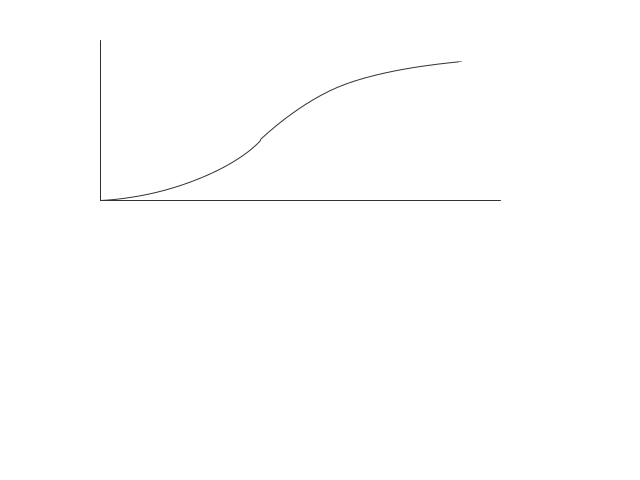
\includegraphics[width=0.8\hsize,trim=2cm 4cm 7cm 1cm,clip]{figures/stable-activity-allocations}
%% }{}

%% Additionally, the problem of the complete diminishing of those activities with longer typical durations, such as home activities, remains the same, when the number and types of activities is flexible.\kai{@Andreas: Naja, das hängt ja eigentlich, wie oben, an der ``utility per typical duration'' und wäre entsprechend einstellbar.  Hat Feil aber wohl nicht gemacht.}

%% It might be worth to take another approach based on the observation of \citet[][]{SchlichEtAl_TransportRev_2004} and others, which is that activity, location and mode together form packages that are rarely changed. 
%% One could think of the optimization task as a knapsack problem, where the traveler creates a Gestalt \kai{Kann man das sagen?  Im Bereich der Philosophie ok, aber im Engineering?} of the interactions to satisfy his commitments and his desires. 
%% \gls{tasha} is a model that takes a similar stance. 

%% \gunnar{? Als ``reality check'' sollte man sich vielleicht fragen, ob Eric Miller hier nicken w\"urde..}

%% % ---------------------------
%% \ah{see also: Vaibhav Srivastavaa, Francesco Bullob, Knapsack Problems with Sigmoid Utilities: Approximation Algorithms via Hybrid Optimization, Section~3
%% }

%% \createfigure%
%% {\ah{temporary (for me to get a picture of what is happening): ``surviving'' convex acts}}%
%% {\ah{temporary (for me to get a picture of what is happening): ``surviving'' convex acts}}%
%% {\label{fig:zhnetwork}}%
%% {%
%%   \createsubfigure%
%%   {Case~2 as in Figure~\ref{fig:unstable-activity-allocation}}%
%%   {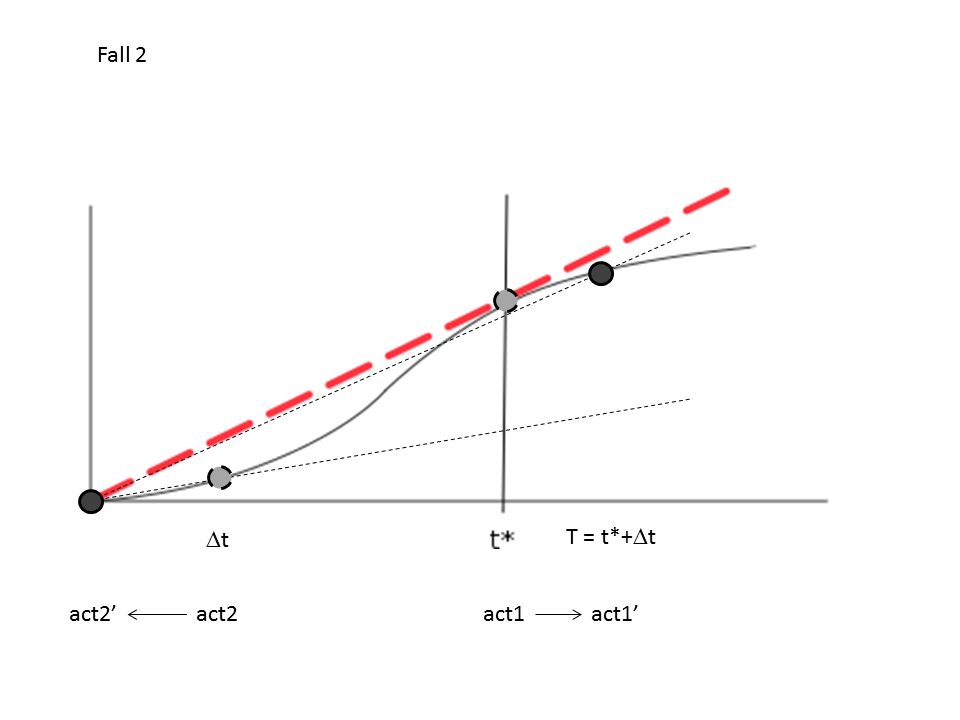
\includegraphics[width=0.8\textwidth,angle=0]{figures/tmp_case2}}%
%%   {\label{fig:tmp_case2}}%
%%   {}%
%%   \createsubfigure%
%%   {Case~3 (sigmoid?)}%
%% 	{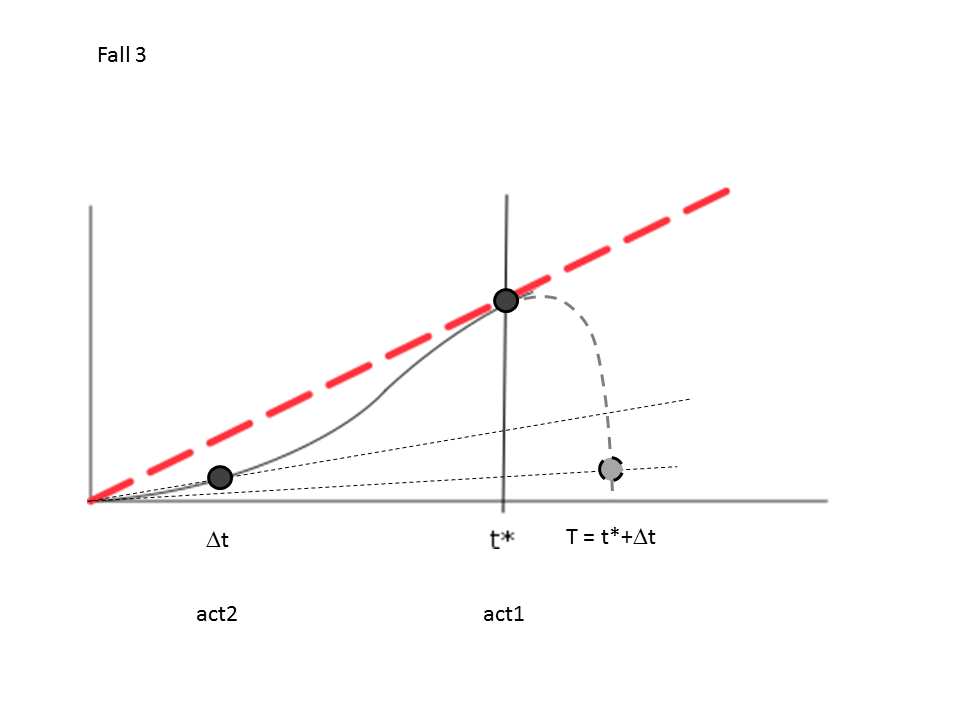
\includegraphics[width=0.8\textwidth,angle=0]{figures/tmp_case3}}%
%%   {\label{fig:tmp_case3}}%
%%   {}%
%% }%
%% {}

%% % ---------------------------
%% \paragraph{Polynomial of Second Degree}

%% It was explained above (Section~\ref{sec:discussion-present-math-form}) that a problem with the present functional form, $\beta_{perf} \cdot t_{typ,q} \cdot \ln( t_{dur,q} / t_{0,q} )$, is that activity durations shrink proportionally when a person gets under time pressure, and sometimes this may not be plausible, for example when attempting to maintain 8~hours of work per day.  The mathematical problem behind this is that the curvature of the scoring function at the typical duration cannot be separately controlled for the different activity types.  This becomes clear when taking derivatives:
%% \[\begin{matrix}
%% S'_{act,q} & = & \beta_{perf} \cdot t_{typ,q} / t_{dur,q}
%% \qquad
%% & \hbox{ and thus } &
%% \quad
%% S'_{act,q} \Big|_{t_{dur,q} = t_{typ,q}} & = & \beta_{perf}
%% \\
%% S''_{act,q} & = & - \beta_{perf} \cdot t_{typ,q} / t_{dur,q}^{-2}
%% \qquad
%% & \hbox{ and thus } &
%% \quad
%% S''_{act,q} \Big|_{t_{dur,q} = t_{typ,q}} & = & - \beta_{perf} / t_{typ,q} \ .
%% \\
%% \end{matrix}\]
%% That is, since $t_{typ,q}$ needs to be used to define the duration where the scoring function has slope $\beta_{perf}$, there is no parameter left to set the second derivative and thus the curvature of each activity type separately.  In consequence, the current form of the \gls{matsim} scoring function allows no control over how flexible an activity is.

%% The above indicates that one may want to control for height, slope, and curvature at the typical duration.  This implies that one might want to try a polynomial of second degree, i.e., $S_{act,q} = A \, t_{dur,q}^2 + B \, t_{dur,q} + C$, with the following conditions:
%% \[\begin{matrix}
%% S_{act,q} \Big|_{t_{dur,q}=t_{typ,q}} & \stackrel!= & const \cdot t_{typ,q} \\
%% S'_{act,q} \Big|_{t_{dur,q}=t_{typ,q}} & \stackrel!= & \beta_{perf} \\
%% S''_{act,q} \Big|_{t_{dur,q}=t_{typ,q}} & \stackrel!= & \gamma \\
%% \end{matrix}\]
%% Solving leads to
%% \[
%% S_{act,q} = \frac{1}{2} \, \gamma \, t_{dur,q}^2
%% %
%% + \Big(- \gamma \, t_{typ,q} + \beta_{perf} \Big) \, t_{dur,q}
%% %
%% + \Big( \frac{1}{2} \, \gamma \, t_{typ,q}^2 - \beta_{perf} \, t_{typ,q} + const \cdot t_{typ,q} \Big) \ ,
%% \]
%% which is, in fact, more expressive than it looks at first glance:
%% \begin{itemize}

%% \item $\frac{1}{2} \, \gamma$ in the quadratic term is just there to generate the requested second derivative.

%% \item $\beta_{perf}$ in the linear term is there to generate the requested slope at $t_{typ,q}$; $- \gamma \, t_{typ,q}$ is there to compensate the contribution of the quadratic term at the same point.

%% \item Similarly, $\frac{1}{2} \, \gamma \, t_{typ,q}^2 - \beta_{perf} \, t_{typ,q}$ in the constant term are there to compensate for the higher order contributions at $t_{typ,q}$; once that compensation has taken place, $const \cdot t_{typ,q}$ is the term that determines the ``height'' of the scoring function at $t_{dur,q} = t_{typ,q}$.

%% \end{itemize}
%% An additional advantage of the 2nd degree polynomial would be that a separate linear extension for negative durations (\cf Section~\ref{sec:negative-durations}) would no longer be necessary. 
%% %
%% Overall, it seems that such a scoring function should be investigated for \gls{matsim}.

%\gunnar{Warum nicht die regelbasierten Systeme 
%von Miller oder Arentze laufen lassen und dann eine utility-function suchen, welche die simulierten Pr\"aferenzen 
%reproduziert? Da kann man dann ja beliebig viele Daten erzeugen und vielleicht sogar nicht-parametrische 
%utility-Funktionen plotten.} 
%\kai{@Gunnar: Ja, warum nicht? Willst Du es als research avenue aufschreiben?}
%\ah{Offenbar nicht. Vielleicht in der nächsten Edition.}

% ---------------------------------------------------------------------------------------------------------
%\subsubsection{Stability Issues With the S-Shaped Function}
%\label{sec:stabilityissues}

% ----------------------
%\ah{Some pieces of notes: Cannot put it down:
%
%Furthermore, an optimum with activity durations in the convex region of their utility functions is unstable. 
%...
%
%Either, (a) a small increase of their durations generates larger overall utility, than the shortening of the remaining activities in the concave region. Then the increasing curvature lets this activity increase further, or (b) the shortening 
%
%Furthermore, there are points where common system stability criteria---small perturbations only have small effects---is broken.
%At such points of the optimization trajectory, for filling up the time budget, it is suddenly better to add a new activity to the convex region than to prolong an activity in the concave region. \ah{ist immer so bei act repl}
%Due to the the S-shaped function's symmetry \ah{explain...symmetry not correct}, these points seem to fall together with the inflection points of the the bell-shaped first derivative of the S-shaped function.
%
% The optimization problem however, does neither have a stable optimum. An S-shaped function's first derivative is bell-shaped, \ie not bijective,
%
%The optimum is only kept, in the rare case, where the budget constraint exactly matches with all activities being at their utility function's inflection point, where the marginal utility is maximal.
%In all other cases ...
 %
%The maximum marginal utility is at the inflection point.
%
% The log forms first derivative $1/x$ is bijective.
%
%Together with the flexible number of activities, this means that there are infinitely many optima, \ie
%the time budget $T$ can be assigned to a variable number of activities in infinitely many ways representing an optimal plateau.
%
%with $N$ activities of which $m$ activities lie below injection point with first derivative $\cdot{f_0}$ and $N-m$ activities lie above injection point with first derivative $\cdot{f_1}$, 
%the total time budget $T$,
%and the infinitely small time change $dt$ 
%\begin{equation}
%m \cdot \dot{f_0}(t_0) \cdot dt = (N-m) \cdot \dot{f_1}(t_1) \cdot (T-m\cdot dt)/(N-m)
%\end{equation}
%has infinitely many solutions as $N$, $t_0$, $t_1$ are flexible; $t_0$ and $t_1$ are dependent on each other though.
%This also includes the case that activities have zero durations.
%In any case, it is very difficult to estimate such a function.
%Its behavioral suitability is another unsolved issue.
%
%\ah{ungewöhnliche Notation mit $dt$, wie schreibt man das sonst?}
%
%-------------
%
%consumer theory, first derivative equal -> defined clear optimization problem. 
%
%In other words, first derivatives do not need to be equal, 
%
%various combinations of activities lying above utility function injection point while others are below it are possible.
%
%This means that as long as the number of activities is flexible (degree of freedom) there exist ...
%
%The system is only stable (and optimal) if all non-zero-duration activities are exactly at inflection point of the utility function as detailed by following differentiation: 
%\begin{enumerate}
%\item All activities are in concave region (thus having equal marginal utility). Adding another activity might add additional benefit. 
%\item All activities are in convex region (thus having equal marginal utility). Removing one activity might add additional benefit.
%\item Some activities are in convex and others are in concave region. Increasing the convex activities while reducing the concave activities, or the other way round, might generate additional benefit.
%\end{enumerate}
%
%If one activity duration was in the convex region, then the overall utility could be increased by either
%(i) increasing its duration and at the same time reducing the duration of one activity in the concave region, or
%(ii) decreasing its duration and at the same time increasing the duration of one or more activities in the concave region.
%
%In any case; alle Ableitungen gleich stimmt nicht mehr
%
%If all activity durations are in the concave region (negative second derivative), another activity is added.
%If all activity durations are in the convex region (positive second derivative), at least one activity is set to zero 
%
%
%It does, however not prevent activities being set to zero duration.
%
%intuitively assigns the function estimates too much power.
%
%Problematic with this approach is the fact, that the system is only one stable point, the inflection point. 
%
%For the log function and at the optimal point all marginal utilities are equal. 
%
%Metaphorically speaking, the agent performs a system optimum search in terms of assigning time budgets to activities, where here system optimum is congruent with user optimum.
%
%
%For the S-shaped function system optimum is not necessarily congruent with user optimum, meaning that not all activities have equal marginal utilities at the system optimum point.
%
%In case the overall budget is too small to have all activities located in the concave region, there will be 
%
%There is no stable point in the convex region however. A stable point has $n$ activities in the concave region and $m$ activities at zero. 
%
%The gradient is positive but diminishing (second derivative negative). The system optimum view is congruent with the user optimum view.
%
%In the convex region. system optimum. Not all activities equal. gradient positive and increasing (second derivative positive). Pushed to zero nevertheless, if remaining activities in convex region generate more utility! Large depends on estimation. Only works correct in concave region.
%
%This is not a Lennard-Jones force!
%}

% ---------------------------------------------------------------------------------------
%\kai{Hallo Kay,
%Ist Euch die S-shaped utl function so wichtig, dass Ihr sie im "Buch" stehen haben wollt?
%Meine Intuition ist nämlich folgende:
%Es herrscht Wettbewerb zwischen Aktivitäten.
%Optimal ist wenn alle ersten Ableitungen nach der Zeit identisch (wie bei normaler consumer theory Ableitungen nach dem Preis).
%Theoretisch kann damit ein Arbeitspunkt auch im konvexen Teil der utl fct liegen.  Das ist aber instabil (siehe PS), und wird sich daher immer entweder nach Null oder in den konkaven Bereich bewegen.
%Damit gibt es aber auch in der Realität nur wenig oder gar keine Dauern im konvexen Bereich.
%Damit ist der konvexe Bereich nicht schätzbar.
%Insofern waren die Probleme bei Feil hier m.E. nicht Pech, sondern systematisch.
%Von mir aus kann sich die Welt damit trotzdem beschäftigen.
%Aber soll es wirklich als "research avenue" in das MATSim-Buch?  Oder könnten wir uns auf eine allgemeinere Formulierung einigen (wo wir einfach sagen, dass die derzeitige matsim fct zu unflexibel ist)?
%Danke \& vG
%Kai
%%
%PS: "Instabil": Sobald der Arbeitspunkt hier etwas nach rechts geht, geht die Steigung nach oben, der marginale Zugewinn steigt also an.  
%- Falls dieser Gewinn an Steigung mehr ist als der Verlust an Steigung an allen anderen Aktivitäten, dann wird der Anteil der betrachteten Aktivität immer größer, bis der Arbeitspunkt im konkaven Bereich ist.
%- Falls nicht, so gilt das Argument andersherum, und die betrachtete Aktivität wird auf Dauer Null zusammenschnurren.
%}

%\kai{Wir können aber auch unter research avenues durchaus so etwas wie "alternative functional forms of the utl function" als Überschrift nehmen, und dann kurz erklären, dass Feil es mit der Joh-Fkt probiert hat, aber mit einem Teil der Parameter Schätzprobleme hatte.  M.E. sollte nur das mit dem S nicht in der Überschrift stehen.}

% diminishing returns ... negative 2nd derivative

% prudence ... positive 3rd derivative --> 2nd derivative goes up (but has to stay below zero because of point above)

% =========================================================================================
\subsection{Heterogeneity of Alternatives and Challenges of Estimation}
\label{sec:estimation}

It is common to differentiate between types of alternatives in the average; for example, trips by different modes or with different purposes are commonly assigned different values of time.
%
However, there are also large deviations from those averages between travelers.
%
A possible approach to address that are so-called taste variations, \ie to make some parameters of the utility function random but fixed per agent, and the parameters of this randomness are made part of the choice model estimation.
%
However, some of this apparent randomness may, in fact, be causal.
%
For example, higher values of time for commuting than for leisure may be caused by the more crowded daily schedule on working days.  Similarly, the strength of a preference for public transit may be caused by the walking distance to that transit stop that serves the desired destination.

Simulation systems such as \gls{matsim} should be able to explicitly integrate such heterogeneity of the alternatives.  
Besides the aspects discussed in 
%Section~\ref{sec:alternative-functions}, 
Section~\ref{sec:future-of-scoring-function},
it is desirable to know how the following aspects influence the scoring function:
\begin{itemize}

\item Access/egress times to/from public transit.

\item Transfers between public transit lines.

\item Crowding in public transit vehicles.

\item Parking search.

\item Types of parking (on-street, guarded, sheltered, etc.)

\item Personal or household income

\end{itemize}
Clearly, this list is not complete.

For most of these aspects, initial studies within the \gls{matsim} context are available, see, e.g.\ 
%
\citet{MoyoNagelptLineCalibration,MoyoNagelptNetCalibration} for access/egress times and transfers to \acrfull{pt}, 
%
\citet{BoumanEtc2013Crowdedness} 
\kai{some Singapore ref?} 
\kai{Hallo Alex, Könntet Ihr uns bitte eine Referenz aus Eurer Arbeitsgruppe für die Untersuchung von pt crowdedness im Kontext des folgenden Satzes empfehlen: [...]}
for crowdedness,
%
\cite{WaraichEtAl_STRC_2013} for parking search,
%
or \cite{KickhoeferEtAl_Transportation_2011} for income.
%
In some cases, it is even possible to configure these elements through the standard config file, completely without \gls{java} programming.
%
It is also quite clear that these issues were addressed outside the \gls{matsim} context.
%
A challenge, however, is that it is normally not possible to just collect and combine results from different studies, for the following reasons:
\begin{itemize}

\item It is not correct to take an estimated utility function and then change the list of attributes.  
%
For example, if walking access/egress to/from \gls{pt} is not included in the estimation, then its effect may be partially be included in the alternative-specific constant or in the population density (which may serve as a proxy for the density of \gls{pt} access points).  Just adding the effect of walking access/egress from some other study is thus not correct.

\item Even when \gls{matsim} is able \emph{in principle} to add these elements, doing so in practice poses a considerable statistical challenge.  For example, one may assume that households inside a zone self-select their precise residential location based on the \gls{pt} accessibility of their regular destinations.  
%
In contrast, a typical \gls{matsim} initial demand generation process will first assign residential locations, and then generate their destinations, e.g.\ their workplaces.
%
In consequence, persons who might reach their destinations easily by \gls{pt} might have their \gls{matsim} residences far away from the relevant \gls{pt} stop.

\end{itemize}

It is thus necessary to estimate the scoring function with exactly those attributes that are available in the simulation in sufficient precision.
%
\citet[][]{Kickhoefer_MastersThesis_2009} has, in consequence, re-estimated his scoring function based on data from \citet[][]{VrticEtc2008ReisekostenSVIBericht}. 
%
For the same reasons, it is not possible to combine functions that were independently estimated for different choice dimensions.  This is not even possible when they all contain monetary units.  For example, assume that one has
\[
... + \beta_{t} \, t_{trav} + \beta_{m} \, cost + ...
\]
for mode choice, and
\[
... + \beta_r \, \rho + \tilde\beta_{m} \, cost + ...
\]
for parking, where $t_{trav}$ is the travel time, $\rho$ is the crowdedness of a parking lot, and $cost$ is in all cases the monetary cost, \eg for gas, \gls{pt} fare, or parking.  Even then it is not possible to say
\[
... + \beta_{t} \, t_{trav} + \beta_{m} \, cost 
%
+ \beta_r \, \frac{\beta_m}{\tilde\beta_m} \, \rho + ... \ ,
\]
since that confuses the scale parameters of the two separate estimations.% 
%\gunnar{b' war im eco-Kapitel die Zeitableitung von b.}
\footnote{%
%
Although, realistically, combining separate estimations via their conversion in monetary terms may be the best one can do in many situations.
%
} If only travel time is available as common attribute, the situation gets worse, since the valuation of time in \gls{matsim} is non-linear, and thus operating points for linearization need to be defined, or found by iterative procedures~\citep[][p.75ff]{Horni_PhDThesis_2013}.

As a long-term perspective, one could also imagine to estimate the choice models directly inside \gls{matsim}, possibly taking hints from \acrshort{urbansim} (\acrlong{urbansim}) which has such an approach at its core.  An early step in this direction within \gls{matsim}, using \acrshort{cadyts} (\acrlong{cadyts}; Chapter~\ref{ch:cadyts}), is described by \citet{FloetteroedChenNagel2012ChoiceModelRefinement}.

% \gunnar{Im Prinzip kann man inzwischen alles sch\"atzen, was man auch simulieren kann. Techniken wie Indirect Inference
% machen das m\"oglich. Das Problem sind ``nur noch'' die weiterhin exzessiven Rechenzeiten. Eine langfristige Perspektive
% ist daher, die choice models in der Simulation zu belassen, wenn man sie sch\"atzt, insbesondere also auch die Attribute
% der Alternativen endogen zu simulieren. Damit hat man dann auch ``automatisch'' Konsistenz zwischen dem, was man sch\"atzt
% und dem, was man simuliert. Ich meine mich zu erinnern, dass das GUI von Urbansim auf der gleichen \"Uberlegung aufbaut,
% indem es Sch\"atzung und Vorhersage in einen Arbeitsablauf integriert.}
% 
% \kai{@gunnar: habe mal zwei Sätze in diese Richtung geschrieben.  Ok mit dem Floetteroed et al paper?}



%% %as well as missing interactions with the trip purpose 
%% %Mir nicht wirklich klar. Beispiel?  Oder einfach weglassen.
%% An additional complication, in particular with respect to monetary items, arises from
%% %and the 
%% often omitted or misspecified 
%% %distribution 
%% assignments of the payment responsibilities (the firm paying, the parents paying for young adults, girlfriends paying for their boyfriends etc.).  However, not all differences stem from the context, and in consequences the following elements should be investigated concerning their explanatory power for a possible inclusion into the \gls{matsim} scoring function:
%% %% Still, the following differences should be accounted for:
%% %
%% \begin{itemize}\styleItemize
%% \item Modal preferences, which could, for example, be included as \kai{person-specific???} modal constants or as \kai{person-specific??} mode-specific valuation of in-vehicle-travel times to capture the comfort and social prestige effects
%% \item Walking time \kai{Das erscheint mir im Hinblick auf den bereits bestehenden matsim-Status zu unpräzise, da ``walking'' in matsim schon lange drin ist.}
%% \item Transfers as a measure of their inconvenience and risk of the lost connection \kai{Das erscheint mir im Hinblick auf den bereits bestehenden matsim-Status zu unpräzise, da ``transfer'' in matsim schon lange drin ist.}
%% \item Crowding 
%% %above 
%% (in addition to the disutility of the in-vehicle time) %% for its discomfort
%% \kai{Paul Bouman in Rotterdam.  Ist uns leider nie gelungen, das einzufangen}
%% \item Parking search 
%% %above 
%% (in addition to the disutility of in-vehicle time)
%% \kai{Waraich??}
%%  %% for its uncertainty
%% \item 
%% %Type 
%% Preferences for types of parking places 
%% %% for the different levels of personal risk and risk for the vehicle
%% \kai{Waraich??}
%% \item Cost sensitivity, e.g.\ by available personal income 
%% \kai{Kickhoefer??}
%% %% \item Operating points for the activities
%% \item Typical durations of activities by activity type
%% \kai{diese und die nächste stehen etwas ``quer'' im Raum, weil sie sich nicht auf ``zusätzliche Elemente'', sondern auf die allgemeine Parametrisierung beziehen.  Typical durations und ``level'' kann man schon seit Urzeiten kontrollieren; ``curvature'' hingegen fehlt.}
%% \item Level and curvature of the activity utilities by  %% purpose
%% activity type
%% \end{itemize}
%% The literature has shown finer interactions, as well as further elements, but the above set should cover the key parts of the generalized costs. 

%% \kai{Mir ist im Moment nicht klar, was wir mit obiger Liste erreichen wollen, wenn wir für die Hälfte der Items bereits eigene Arbeiten haben.}

%% %As shown earlier, the commonly applied \gls{matsim} utility function parameters are derived from \citet[][]{ArnottEtAl_TAER_1993, ChaumetEtAl_2006}. 
%% \citet[][]{Kickhoefer_MastersThesis_2009} provides estimates based on data from \citet[][]{VrticEtc2008ReisekostenSVIBericht}. 
%% \citet[][]{KickhoeferEtAl2012WelfareBusCorridorKuhmoNectar} translates estimates from \citet[][]{TirachiniEtAl2012CrowdingCongestion} into \gls{matsim} values. 
%% However, with the exception of a few studies \citep[][]{BalmerEtAl_ResRep_datapuls_2010, HuelsmannEtAl2012HotspotPricing, KickhoeferNagel2013EmissionInternalizationNETS, KaddouraEtAl2015PtMarginalSocialCostPricingJTEP}, these estimates have not been considered yet for many other projects, although they represent a valuable base for future comparisons. 
%% The complete set outlined above has not yet been estimated in one consistent estimation, and so remains an urgent item for \gls{matsim} research. 

%% Having such a base at hand is important as estimating and applying a \gls{matsim} utility function is non-trivial due to the following. 

%% %
%% Agents optimize \emph{complete day plans} \citep[see also][Section 6.3.1]{MATSim_Userguide_2015}. This means that the utility levels of the single choice dimensions need to be carefully balanced.
%% %% , when applying estimates. 
%% Usually it is impossible to 
%% apply 
%% %readily-available 
%% functions estimated independently for a single choice dimension. A degenerated example might be the following. All destination alternatives evaluated with a not-well calibrated utility function generate very low utility; in that case the complete activity might be simply dropped. 
%% %
%% \benjamin{I dont fully understand the above...what is an inappropriate utility function?} \ah{adapted}
%% %
%% \kai{Finden wir noch ein besseres Beispiel?  Wie sollen, technisch gesehen, ``destinations'' einen zu niedrigen Nutzen bekommen?  Ich kann mir das nur so vorstellen, dass ein bestimmter Aktivitäten-Typ im Mittel einen zu niedrigen Nutzen bekommt.  Das ist dann aber das gleiche Problem wie oben für activity dropping bereits diskutiert.}
%% %
%% This correlation or dependency between choice dimensions is also the reason why a day plan equilibrium does not necessarily include a Nash equilibrium for every single choice dimensions. 
%% %
%% \kai{Warum nicht?  Wenn ich zwei Pläne haben, die sich in einer choice dimension unterscheiden, dann wechsle ich zur besseren Alternative.  Auf diese Weise sind irgendwann alle choice dimensions im NGG. Was übersehe ich?}
%% %
%% The inseparability of choice dimensions means that in \gls{matsim} we can only consistently handle choices if the parameters are estimated or postulated consistently. 
%% Estimates from independent studies reflect the scale parameter of the Gumbel distribution of the observed choices, which is arbitrarily set to zero \kai{one??} for identification purposes, which means that the values cannot be compared 
%% %\kwaah{(See Bierlaire, ????)}
%% . The elasticities and trade-offs values can be compared, as they removed the scale parameter from their values. 
%% %
%% \benjamin{Why? The only difference if one has more choice dimensions in the model is that utility differences resulting from some policy will be smaller than with less choice dimensions---\ie influencing the elasticity.} \ah{adapted}

%% Incorporating a contribution, \eg for parking or destination choice, in combination with absolute utilities is even trickier as the Charypar-Nagel function is non-linear, which means that available parameters---very often linear utility functions---need to be incorporated by approximation procedures and distinction of cases as described in \citet[][p.75ff]{Horni_PhDThesis_2013}. 
%% Furthermore, \gls{matsim} utility function includes travel times, while their parameters which are readily available from studies, the quality and potential bias in the calculation of the travel times used for those estimate is rarely challenged. 
%% It would be unlikely that these estimates are perfect, given that disaggregate assignment models have until recently only been calibrated against counts and not against observed travel times. 
%% The omission of junction models cannot help either. 
%% In addition, the travel time estimates are influenced by the underlying mode choice model in that implementation which can bias the results further \citep[][]{Vrtic_PhDThesis_2003}. 
%% \gls{gps} or smartphone-based surveys, however, provide this information with higher precision and, thus, they are a promising mean for better model calibration and therefore better description of the non-chosen alternatives in the model .

%% Furthermore, travel time and activity duration parameter estimates including income need to carefully consider the parameters' relation to the \gls{vtts}. \citet[][p.276]{MeisterEtAl_SVT_2009} for example argue that the average Swiss hourly earnings are much higher than 6\,EUR per hour used in the \gls{matsim} function then. 
%% However, the \gls{matsim} is now measured in utils not monetary units. 
%% Still, the parameters in utils and monetary terms (such as tolls, parking costs, fares etc., or income-dependent attributes) are often interacted and thus their relation needs to be consistent if they come from different studies.
%% %
%% \benjamin{I dont see the problem here...parameters define the \gls{vtts}, and are dependent on the variance of the unobserved attributes, no? So measuring in utils or money does not make a difference.} \ah{adapted}

%% %A numerical problem, particularly relevant for activity choice, concerns the functional form of the utility function---As argued in Section~\ref{sec:alternative-functions}, a function offering an additional degree of freedom (the curvature at the typical duration) would be better.

%% Estimating a utility function for \gls{matsim} is associated with another problem. 
%% The function is applied iteratively for a travel demand, which is in the beginning of the relaxation process usually not very similar to the situation for which the function was estimated. 
%% In other words, the function is used for a whole range of operating points, whereas it has been estimated for only one possibly completely different working point. 
%% The \gls{matsim} function thus must be also correct in the elasticities, to be able to efficiently drive the relaxation process toward the final relaxation point, where the estimated function is valid by construction. 

% =========================================================================================
\subsection{Agent-Specific Preferences}
\label{sec:agent-specific-prefs}
\gls{matsim} scenarios so far consider a relatively small set of agent attributes, essentially because of missing suitable data to derive detailed attributes for large populations \citep[][]{MuellerFloetteroed_unpub_hEART_2014}. 
Some studies, however, used larger sets of attributes. 
\citet{GretherEtAl2010TrbIncomeInTRR, KickhoeferEtAl_Transportation_2011} estimated individual income-contingent utility functions. 
\citet[][]{HorniEtAl_TechRep_IVT_2012_a, HorniAxhausen_TechRep_IVT_2014} incorporated agent-specific travel preferences and individual income-dependent marginal utilities of money; the preference values, however, were assigned randomly. 
As natural consideration of agent-specific preferences is one of the corner-stones of agent-based \glspl{microsimulation}, future work should exploit this avenue. 

%\benjamin{Das haben wir auch gemacht -- vielleicht sogar noch ein bisschen genauer (mit HH-Einkommen und Lorenzkurve). Siehe \cite{GretherEtAl2010TrbIncomeInTRR, KickhoeferEtAl2011PolicyEvaluationIncome}. Da das früher war, vielleicht hier reinnehmen?} \ah{done}

% =========================================================================================
\subsection{Frozen Randomness for Other Choice Dimensions Than Destination Choice}
\label{sec:future-frozen-randomness}

For destination choice an iteration-stable random error term has been successfully applied to incorporate the unobserved heterogeneity not included by the stochasticity of the co-evolutionary process (see Chapter~\ref{ch:destinationchoice}). Other choice dimensions
%, already implemented but in particular, future implementations concerning activity choice 
might also benefit from explicit agent-specific error terms.  
%% A general implementation would obviously be useful. 
This 
%implementation 
could incorporate a mechanism to generate the error terms with the correct correlation structures. 

%\gunnar{Siehe diesbez\"ugliche Kommentare im eco-Kapitel.}
%\ah{diese Diskussion muss jetzt endlich mal ein Ende finden hier und kann in Edition 2 weiter vertieft werden.}

More formally: 
%
The current \gls{matsim} choice process can be interpreted as maximizing, for each agent $n$, 
\[
U_{ni} = V_{ni} + \tilde V_{ni} + \vec{\beta}^T \vec{\eta_{ni}} + \tilde \eps_{ni} \ ,
\]
where 
%
$V_{ni}$ is the systematic utility of alternative $i$, 
%
$\tilde V_{ni}$ is a random but fixed (frozen) addition, 
%
$\vec{\beta}^T \vec{\eta_{ni}}$ describes randomness inserted by the network loading model (see Equations~(\ref{eq:score}) and~(\ref{eq:mixture-of-logit})), and $\tilde \eps_{ni}$ is remaining (unexplained) noise.
%
Two challenges are:
\begin{itemize}

\item $\tilde V_{ni}$ denotes aspects that are often assumed as random in choice models, but are fixed in typical \gls{matsim} runs.  An example is the walking distance to the next \gls{pt} stop, which may have to be assumed as random in an estimation context based on travel analysis zones, but which is fixed in the context of a \gls{matsim} run.

$\to$ To be consistent, a choice model and a \gls{matsim} implementation that are used together should use exactly the same disaggregated attributes.

\item In most \gls{matsim} runs, the $\tilde\eps_{ni}$ are either assumed as zero (\lstinline{BestScore}), or are parameterized by the \gls{matsim} choice model (\lstinline{ChangeExpBeta} or \lstinline{SelectExpBeta}), which can be interpreted as that the $\tilde\epsilon_{ni}$ are re-drawn from the distribution every time a choice is made.  This leads, for example, to purely random ``logit'' switchers between a base and a policy case \citep[e.g.][]{GretherEtAl2010TrbIncomeInTRR}.

Moreover, the default plans removal (Sections \ref{sec:plans-removal} and \ref{sec:heterogeneity-in-plans-removal}) has a tendency to remove all alternatives except for the best, effectively setting the $\tilde\eps_{ni}$ to zero for \emph{all} typical \gls{matsim} configurations when run for sufficiently many iterations.

This is acceptable in situations where most of the noise can be assumed to be in the $\tilde V_{ni}$ and/or the $\vec{\beta}^T \vec{\eta_{ni}}$; this may be the case for the choice dimensions of route, mode, and time.  It is clearly wrong for locations, where $\tilde\eps_{ni}$ subsumes preferences that are specific to each person--alternative--pair and that often cannot be included into the $\tilde V_{ni}$.  For example, a person may have a strong preference for ``swimming'' in a situation where the data only knows about ``leisure'' facilities.  In this situation, a possible approach is to generate and random but ``frozen'' $\tilde\eps_{ni}$, as described in Chapter~\ref{ch:destinationchoice}.

$\to$ One should thus evaluate in how far and how a similar approach should be introduced for choice dimensions beyond location choice.

\end{itemize}

\kai{@Benjamin: @Andreas: Neu geschrieben Ende April als Reaktion auf die Tatsache, dass wir es im ``understnanding matsim'' nicht eingefangen kriegen.  To be checked.}


%\vfill\eject
% ##################################################################################################################
\section{Double-Queue Mobsim}
\label{sec:researchavenues-double-queue-mobsim}
The standard \gls{matsim} \gls{mobsim} \gls{qsim} implements a single-queue model as described in Chapter~\ref{ch:kinematicwaves}. The associated \gls{fd} (flow vs. density) is horizontal for medium densities, and falls to zero very steeply at very high densities. This is consistent with the fact that a vehicle leaving a link opens up its space already in the next time step; jam patterns thus have a backwards traveling speed of $L/1\,s$ ($L$ is the length of respective link) rather than the conventional approx.\ 15\,kilometers per hour \citep[see also][]{CharyparEtAl_TRB_2009}. 
%\kwaah{Adding references to Charypar's work on the topic}

The \gls{jdeqsim} (Section~\ref{sec:using-jdeqsim}) and the deprecated \gls{deqsim} (Section~\ref{sec:deqsim}) implement a double-queue model with backward traveling gaps. Currently, implementation work and tests are performed to include this also in \gls{qsim}; performance problems with the inclusion of a large number of ``holes'' is the remaining issue to be solved. \kai{chk before going to print; it may be ok now thanks to Amit}

%\kai{Siehe auch Material in basicprocedure.tex}
%
%Illustrates empirically the summary in Section~\ref{sec:kinematicwaves-summary}.
%\ah{
%\subsection{Aggregate Traffic Flow Characteristics}
%\gls{matsim}'s aggregate traffic flow characteristics were analyzed in the common form of the macroscopic fundamental diagram. Some investigations additionally derived \gls{matsim}'s (implicit) volume-delay function \citep[][]{HorniMontini_STRC_2013}.
%
%Some simulation investigations had problems to reproduce the complete MFD (project NetCap, personal communication, 2014), in particular, the high density region. They used mobsim versions without the backward moving gaps feature. Other studies, based on DEQSim and JDEQSim respectively, which both \emph{do} include \emph{back moving gaps}, were able to generate realistic MFDs. \kai{Das ist natürlich kein Wunder.}
%
%\citet[p.81ff][]{Simoni_MastersThesis_2013} investigates \gls{matsim}'s ability to model macroscopic characteristics with a four link ring scenario. He found considerable influence of the backward moving gaps speed on the form of the MFD. \citet[][]{CharyparEtAl_TRB_2009} also use a circular toy scenario. They also found the typical trapezoidal form for a broad range of network resolutions.
%
%Natural conclusion here is, that back moving gaps are essential for generating a realistic MFD \kai{bis hier hin stimme ich zu}, in other words to realistically model the complete range of traffic conditions \kai{hier eigentlich nicht wirklich.}. Backward moving gaps are re-included in the default \gls{matsim} mobsim (qsim).
%}
%
%\ah{following copied from atlassian:}
%
%\kai{The queue model fundamental diagram (flow vs density) is horizontal for medium densities, and falls to zero very steeply at very high densities.
%This is consistent with the fact that a vehicle leaving a link opens up its space already in the next time step; jam patterns thus have a backwards travelling speed of ``length\_of\_link''/1sec rather than the conventional approx. 15km/h.
%
%A fix, developed by Charypar, is to generate a ``hole'' when a vehicle leaves a link, and have it travel with a configured velocity against the direction of traffic. The hole cannot be used before it has arrived at the upstream end.
%
%Now the problem is that the model is initialized with one hole per empty space. This means many ``hole'' objects which consume a lot of memory ... in fact, too much of it.
%Way out: Just keep track of the number of available holes. Initially, that number corresponds to the storage capacity. Every time a vehicle enters, the number is decreased (which can also take care of different vehicles sizes, \ie decrease by the PCE instead of by one). Every time vehicle leaves, a hole is created (with size equal to the vehicle's PCE) which travels upstream. When the hole has reached the upstream end, the number of available holes is increased accordingly, and the hole object is destroyed.
%This would need to be implemented and tested ...}
%
%\marcel{
%Having the holes only while traveling back brings it closer to an events-based implementation: Basically, the hole then represents nothing else as a delayed event to increase the available space on the link. This leads to a further simplified implementation: Instead of hole objects, one could just have a queue where the time, when an additional space becomes available (=when the hole would reach the start of the link), is stored. In each step, the head of the queue could be checked to see if space becomes available and increase the counter. This would then also be more queue-like like the name of the QSim suggests}
%
%\kai{
%Generelles Problem ist, dass nur die jdeqsim die double-ended queue implementiert, die normale QSim tut das derzeit nicht.  Es gibt seit dem dev mtg eine experimentelle Version für die QSim, aber die verbraucht so viel Speicher, dass man sie nicht empfehlen kann.  Habe jetzt Amit hinzugezogen, damit er mir dabei hilft; keine Ahnung, ab wann wir das evtl. fertig haben könnten.
%}

% ##################################################################################################################
%\section{Synthetic Population Generation}
%Müller
%\ah{not at the core of MATSim, maybe in a next edition}

% ##################################################################################################################
\section{Choice Dimensions, in Particular Expenditure Division}
\label{sec:ra-choice-dimensions}
As shown in Section~\ref{sec:zhgroup_matsim}, and pictured in Figure~\ref{fig:dimensions}, the Zürich group targets at a fuller scheduling model. Besides the standard choice dimensions printed in red in cited figure a bunch of choices is subject to ongoing research. In particular, ``expenditure division'', is untocuhed not only in \gls{matsim} but in transport planning in general as it has focused on single-travelers or household-based groups at most. 
The field's understanding of both the patterns of expenditure and of the styles of allocation inside a household are poor, which is no surprise as the relevant questions are missing in its surveys. 
First tests for the necessary survey works are currently on-going. 
It is expected that this will lead to a better understanding of activity participation and of the values of time travelers bring to their decisions.   

% ##################################################################################################################
\section{Considering Social Contacts}
Apparently, social contacts, within households and within extended social networks have a substantial influence on travel decisions, in particular for social activities in leisure time \citep[][]{KowaldEtAl_unpub_STRC_2009}.
An early social networks study in context but not based on \gls{matsim} is \citet[][]{MarchalNagel_TRR_2005}.
Further work based on or, again, in context of \gls{matsim} was undertaken by \citet[][]{Hackney_PhDThesis_2009, Illenberger2012PhD, IllenbergerEtAl_TechRep_VSP_2010, KowaldEtAl_unpub_STRC_2009, KowaldEtAl_ASNA_2009}.
Most recent work on joint trips is reported in Chapter~\ref{ch:jointtrips}. 
Despite this range of valuable work, future work is required on this topic in particular for leisure destination choice \citep[][]{Horni_PhDThesis_2013}.

%\vfill\eject
% ##################################################################################################################
%\ah{Habe Results' Variability auskomentiert.
%Das Zeug ist nur als STRC-paper publiziert, ist also nichts was die Welt vermissen wird.
%Zudem, ist es mir einfach nicht wohl dabei. Ich habe nicht die geringsten Sicherheiten, dass da nicht noch ein versteckter Bug kräftig mitrauscht.
%Frühere Arbeiten \emph{ohne} Zielwahl kamen auf viel geringere Samplingfehler, also hat man auch durch Kontext keine Anhaltspunkte.
%Zu guter Letzt ist das Ganze jetzt ja zumindest theoretisch in MC abgehandelt.
%}

%\section{Results Variability}
%\label{sec:variability}
%\Gls{microsimulation} system design as well as concrete \gls{microsimulation} studies require specification of the quantities of interest.\footnote{%
%Formal system specification (and verification) is discussed, \eg in \citet[][]{FisherWooldridge_IJCIS_1997, BourahlaBenmohamed_ENTCS_2005}. 
%} For microsimulation design, they need to be general and broadly available, count data are an example. For specific experiments and purposes other measures might be added; \citet[][]{Kitamura_TMIP_1996}, for example, lists measures relevant for emissions modeling. Considering their scale is important for model development, but a certain lack of research exists in this regard. \citet[][Section 2.2]{NagelAxhausen200Xiatbr00-report}, for example, say: ``Another question regarding scales is which scale is necessary to answer which question. There is wide-spread intuition but currently little hard knowledge. Rules-of-thumb, such as to include one level of resolution below the level of interest, are just rule-of-thumb.'' 
%
%Scale of the measures of interest is also relevant for results production, as different scales or resolution levels usually lead to different levels of \emph{variability} and, thus, to different study costs in terms of required computation effort. Transport microsimulations are usually stochastic. Randomness is, for example, introduced by the error terms of discrete choice models, a common component in utility-based \glspl{microsimulation}. This leads to random variability in results. Parameters or population statistics, such as averages, thus, need to be estimated by random sampling. \Glspl{microsimulation} are thus essentially a sampling tool \citep[][]{WolfDA_CSP_2001}, where one run represents one sample unit (in statistical terms one \emph{realization of a random variable}). This makes clear, that the whole toolbox used for other statistical methods, must be applied also here. As a first step, required sample size---here, the number of runs---to ensure a given confidence in the calculated averages needs to be calculated. In this context, variability is often seen as something tedious, because higher variability leads to larger minimal sample sizes, with usually relatively high costs per sample point. But, this view falls short. Clearly, unobserved variability---modeled as random variability---should be replaced to the extent possible (by explaining it). However, when looking at the very large proportion of temporal variability actually present in reality (Figure \ref{fig:counts}), a substantial part of this variability is---even if it was actually explicable---much more efficiently handled by including randomness, as model complexity would be prohibitively large otherwise. In this sense, \glspl{microsimulation} are a tool to capture these real-world fluctuations \citep[][p.11]{NewmanMEJBarkema_1999}, \citep[][p.704]{EsserNagel2001iatbr00-book}. This means also that the focus should not only be on averages, but also on variance incorporated in the calculations of statistical confidence. The following sections broaden the microsimulation variability analysis.
%
%\createfigure[!t!]%
%{Measured volumes}%
%{Volumes. LEFT: Reality.  RIGHT: Simulation. \kai{Hallo Andreas, mitteln die Messungen aus der Realität über alle Tagestypen einschl.\ Samstag, Sonntag, Ostern, Weihnachten, etc.?} \kai{Falls ja, so würde ich sagen, dass das dann ohnehin schwer zu vergleichen ist, und auch erklärt, was man sieht: In den realen Daten vor allem die Schwankungen zwischen den Tagestypen, womit dann die "daily" Schwankungen nicht kleiner sind als die "hourly".  In der Simulation hingegen Monte Carlo noise, der erwarteterweise kleiner wird, wenn man über 24h mittelt.}
%\ah{Die Analyse ist ein Weilchen her. Sehe aber, dass ich die Zähldaten-Dateien für diese Boxplots mit dem gleichen Package (playground.anhorni.counts) erstellt habe, wie die Counts für MATSim. 
%
%Würde also etwas Geld darauf wetten, dass ich auch den gleichen Filter angewendet habe, wie für die Zähldaten (Sa, So, Mo, Fr, Feiertage, Ferien sind somit nicht drin). Argument war damals: Warum um Himmels Willen wollen wir den (Zähldaten-Durchschnitt so genau treffen, wenn wir über mit der Mikrozensus-Nachfrage ein ganzes Jahr reinmixen, was in Realität offensichtlich große Varianz verursacht?
%
%Falls wir es genauer wissen wollen, kann ich das überprüfen/reproduzieren; ist alles als Skript vorhanden.}
%}%
%{\label{fig:counts}}%
%{%
%% ===
	%\createsubfigure%
  %{Daily Volumes}%
%
%{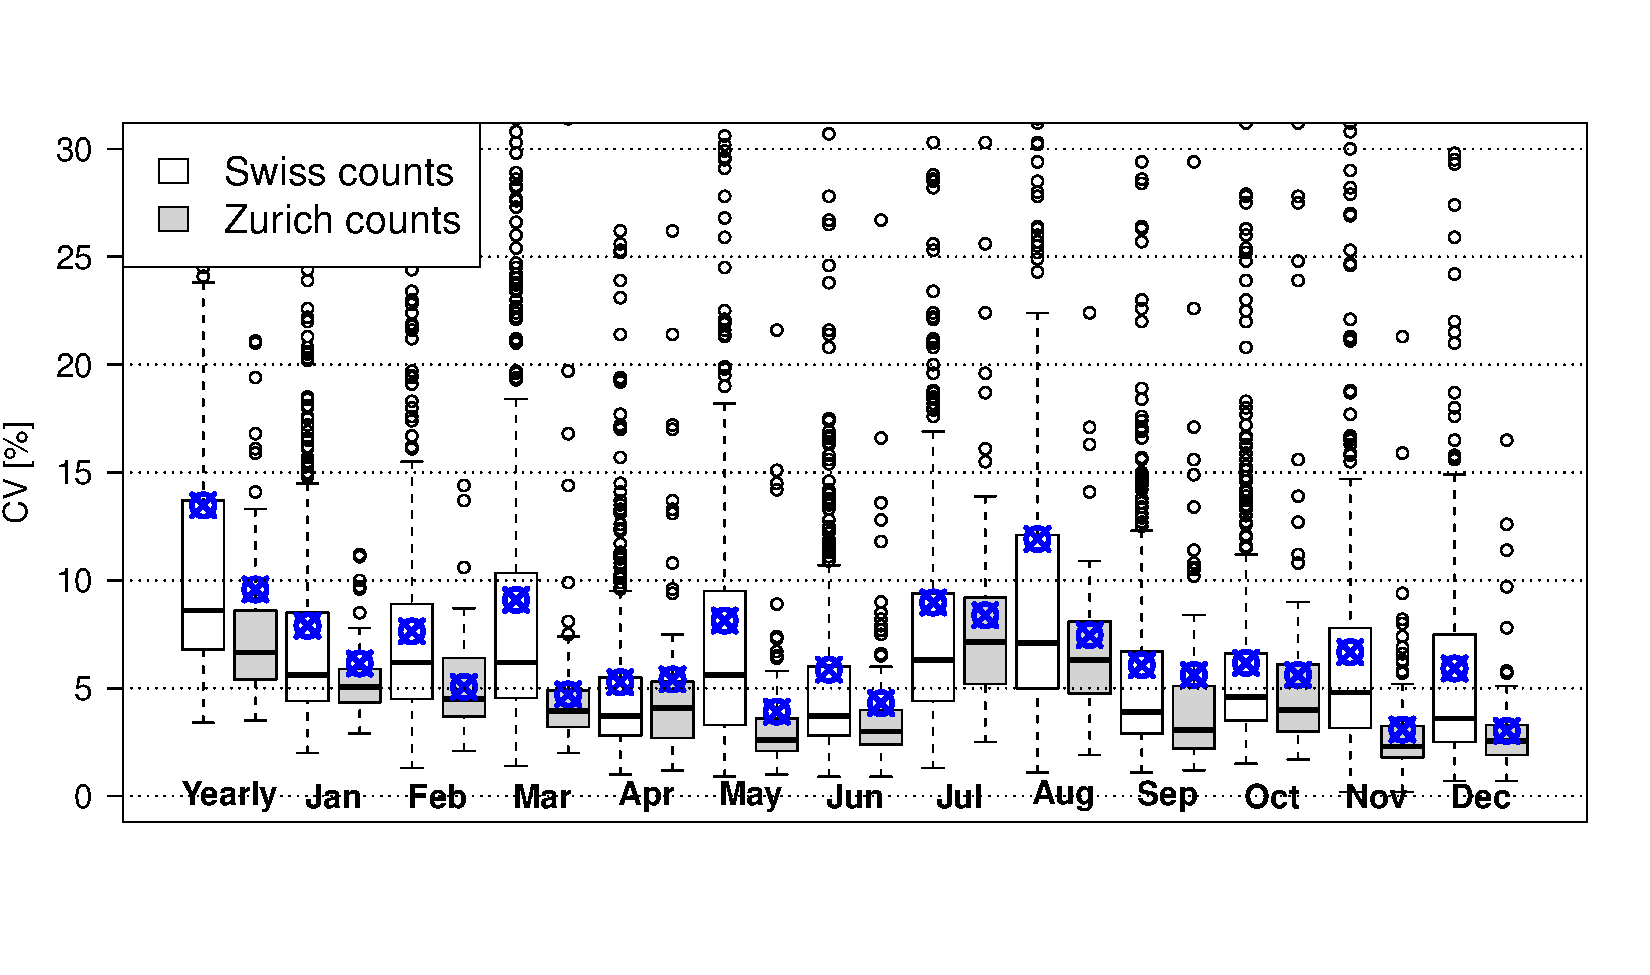
\includegraphics[height=0.3\textwidth]{understanding/figures/var/countsDaily.pdf}}%
	%{\label{fig:countsDaily}}%
  %{}%
%% ---
	%\createsubfigure%
  %{Simulated Daily Volumes: Inter-run Variability, runs~0-29, iteration~200}%
	%{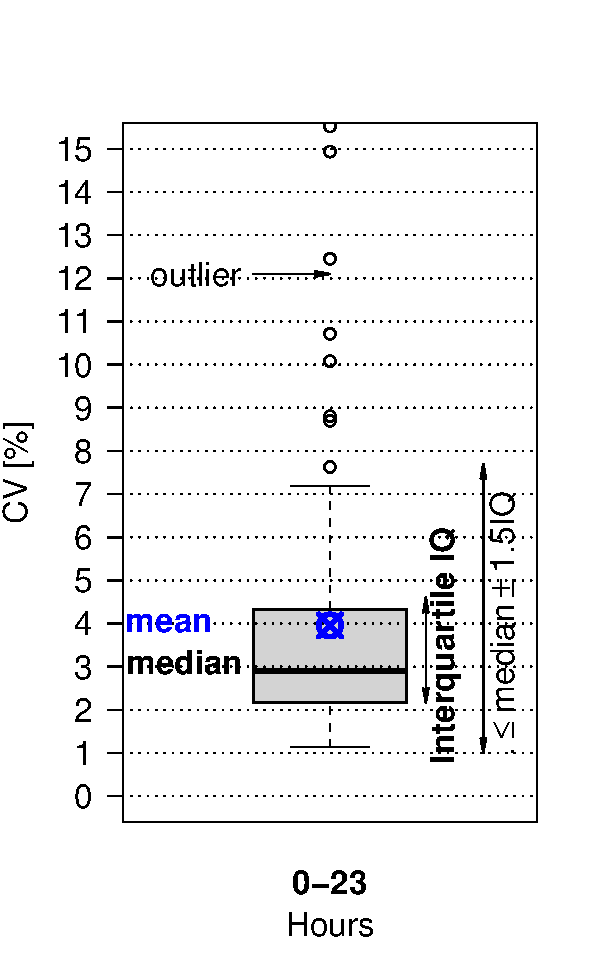
\includegraphics[height=0.3\textwidth]{understanding/figures/var/linkVolumesInterAWTV200.pdf}}%
	%{\label{fig:linkVolumesInterAWTV200}}%
  %{}%
%% ===
  %\createsubfigure%
  %{11:00-12:00}%
	%{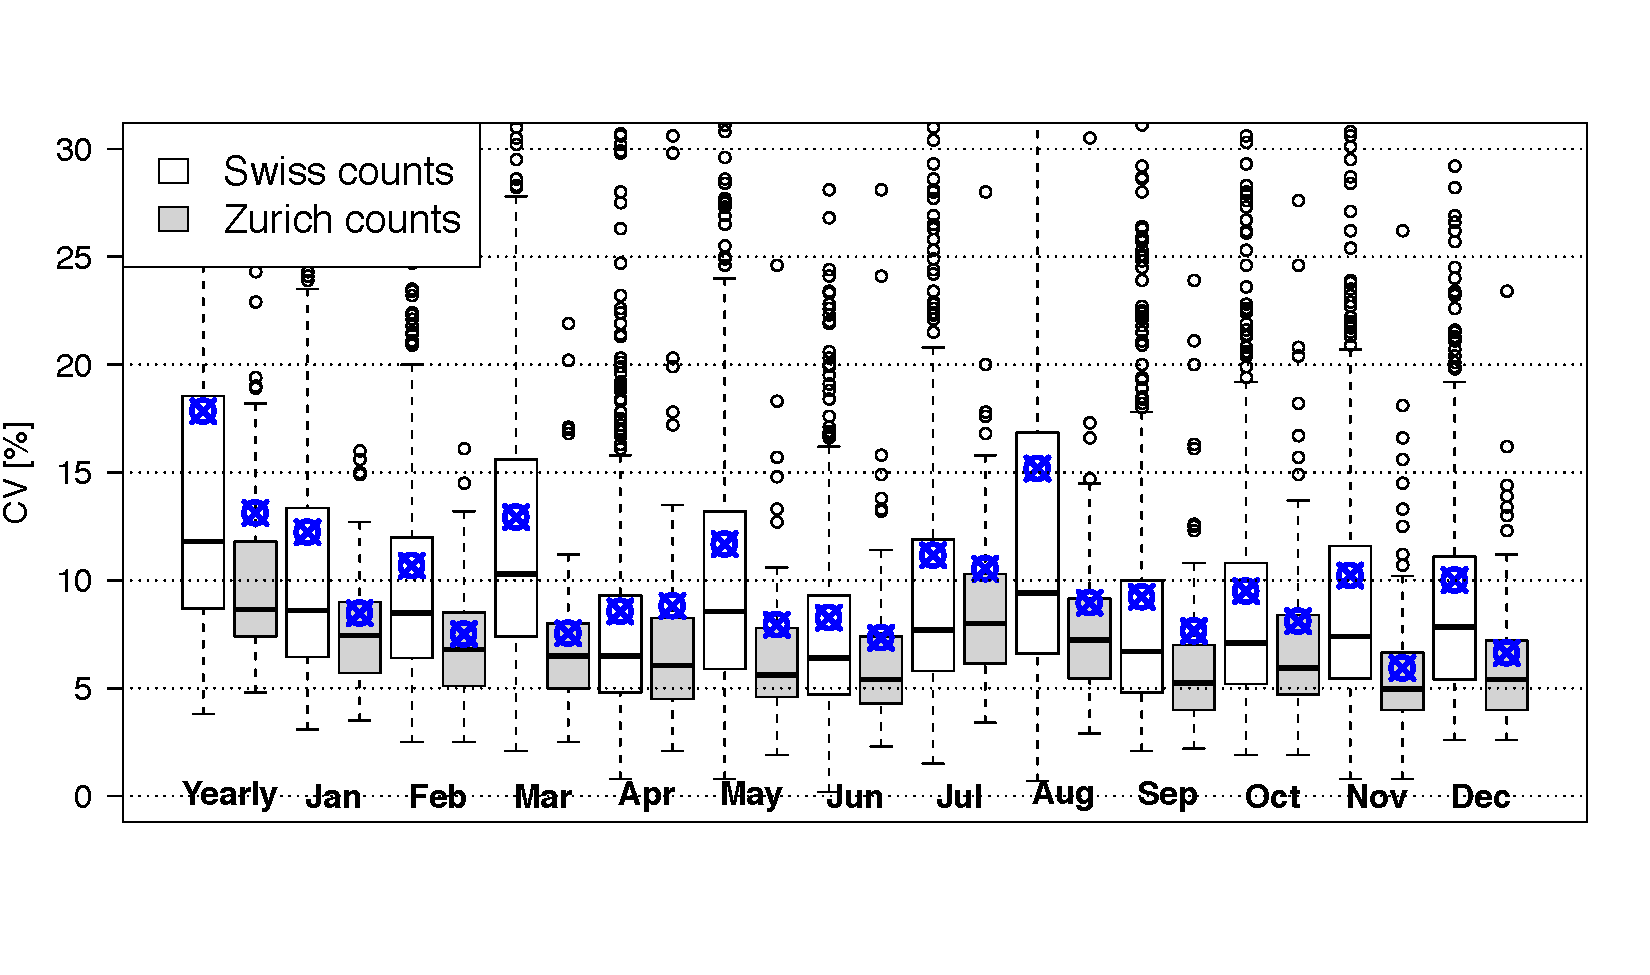
\includegraphics[height=0.3\textwidth]{understanding/figures/var/counts11-12.pdf}}%
	%{\label{fig:H1112}}%
  %{}%
%% ---
	%\createsubfigure%
  %{Simulated Hourly Volumes: Inter-run Variability, runs~0-29, iteration~200}%
	%{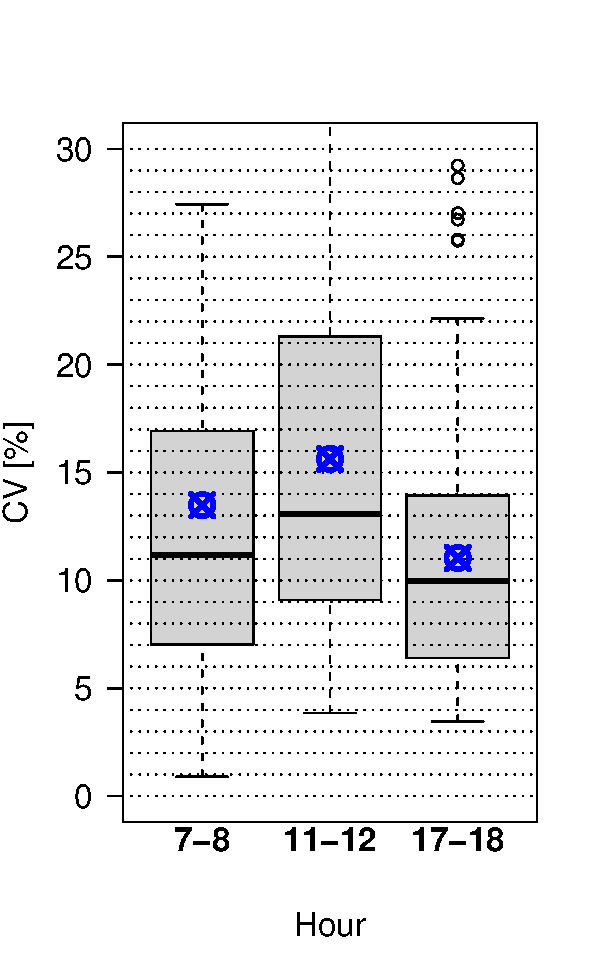
\includegraphics[height=0.3\textwidth]{understanding/figures/var/linkVolumesInter200.pdf}}%
	%{\label{fig:linkVolumesInter200}}%
  %{}%
%% ===
 	%\createsubfigure%
  %{17:00-18:00}%
	%{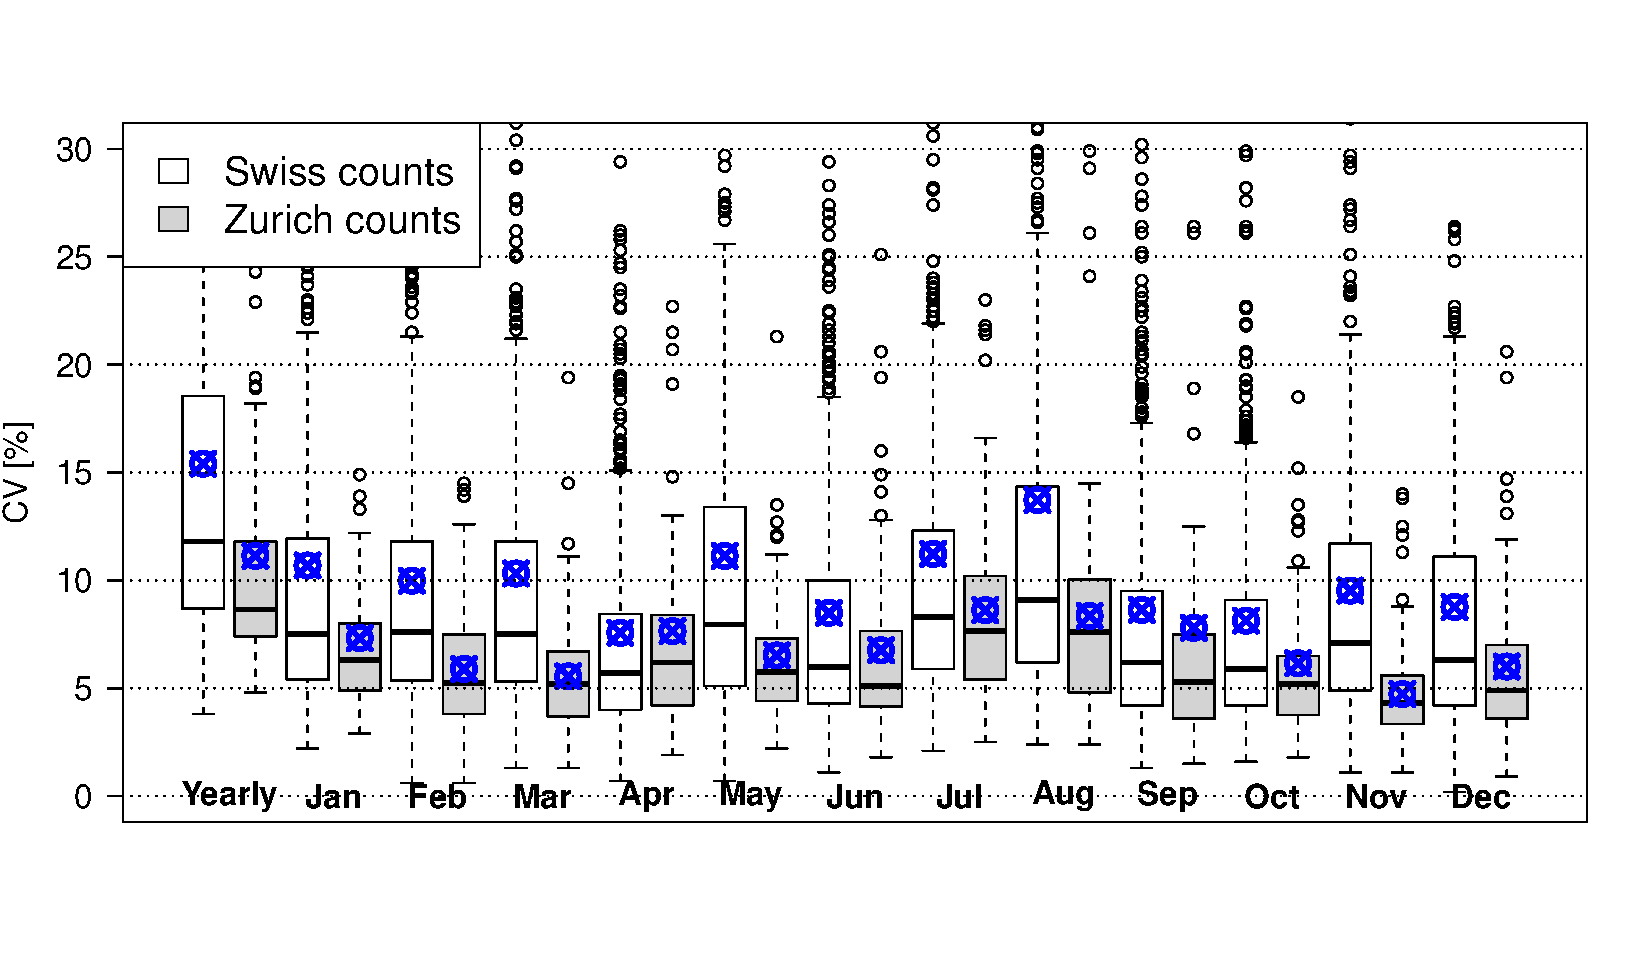
\includegraphics[height=0.3\textwidth]{understanding/figures/var/counts17-18.pdf}}%
	%{\label{fig:H1718}}%
  %{}%
%% ---
	%\createsubfigure%
  %{Simulated Hourly Volumes: Inter-run Variability, runs~0-29, iteration~200}%
	%{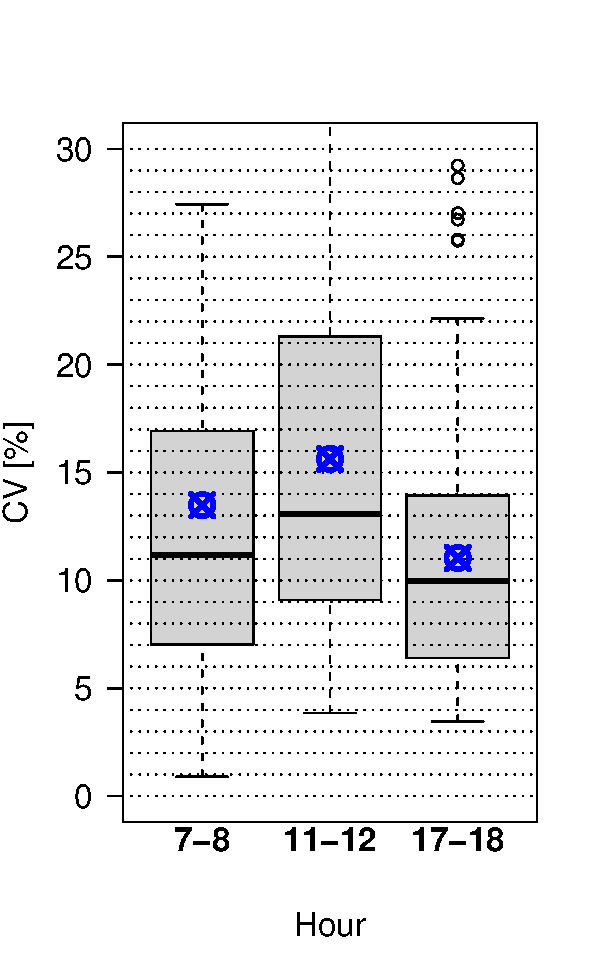
\includegraphics[height=0.3\textwidth]{understanding/figures/var/linkVolumesInter200.pdf}}%
	%{\label{fig:linkVolumesInter200}}%
  %{}%
%% ===
%}%
%{}
%
%Multiple possibilities to categorize microsimulations variability exist; some categories are described by \citet[][]{HorniEtAl_TechRep_IVT_2011_b}. Often a distinction between endogenous (model) variability and exogenous (input) variability is made. Equally suitable one can distinguish systematic and random variability. The experiments reported below mainly focus on \emph{random, endogenous} model variability. Random variability stems from inherently random choices and from actually systematic choices not recognized as systematic by the modeler.
%
%MATSim variability was investigated by \citet[][]{HorniEtAl_TechRep_IVT_2011_b, HorniEtAl_STRC_2011, Dayte_TechRep_IVT_2012} coming to the conclusion that at the population level, as expected, there is little variability between simulation results. Little variability exists likewise for \emph{daily} volumes as shown in Figures \ref{fig:linkVolumesAWTVInterScatter} and \ref{fig:linkVolumesInterAWTV200} (with a different visualization), which is consistent with previous work. However, the variability for \emph{hourly} volumes is an issue as shown in Figures~\ref{fig:linkVolumesHour17-18InterScatter} and Figure~\ref{fig:linkVolumesInter200} (with a different visualization).
%
%To interact these substantial simulation variability with variability observed in reality, \citet[][]{HorniEtAl_STRC_2011} looked at real-world link volumes given for both, the complete year and single months, meaning that a single point in the box plot represents temporal variability of a single network link, either for the whole year, or for a specific month. The hours 11-12 and 17-18 are shown as examples in Figure~\ref{fig:counts}, where similar patterns could be observed for all hours. The plots allow the conclusion that also in reality variability is also substantial.
%
%Further MATSim investigations are reported by \citet[][]{Hackney_PhDThesis_2009, Neumann_PhDThesis_2014}.
%
%\createfigure%
%{Simulated link volumes}%
%{Simulated link volumes}%
%{\label{fig:linkVolumes}}%
%{%
  %\createsubfigure%
  %{Simulated Daily Volumes: Inter-run Variability}%
	%{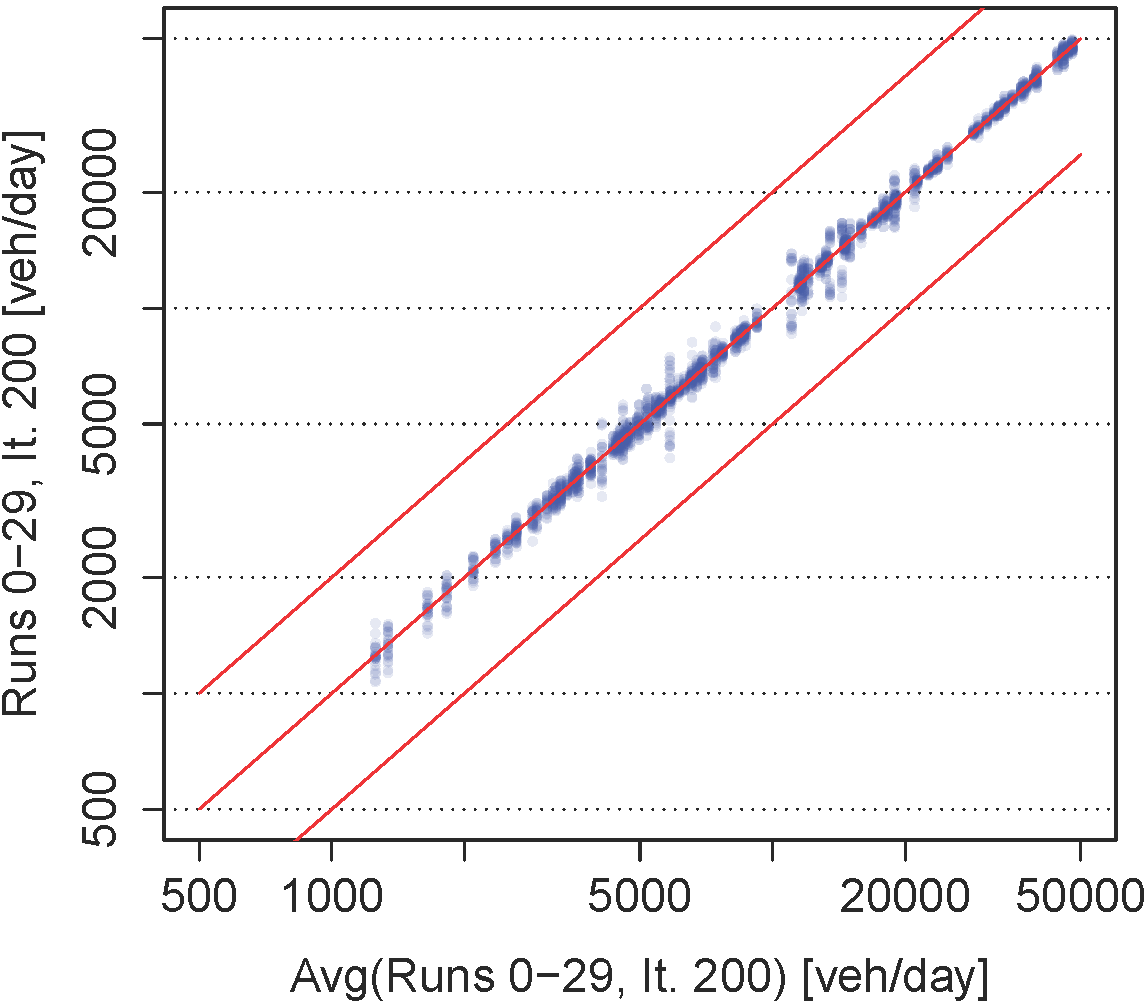
\includegraphics[width=0.49\textwidth]{understanding/figures/var/linkVolumesAWTVInterScatter.png}}%
	%{\label{fig:linkVolumesAWTVInterScatter}}%
  %{}%
	%\createsubfigure%
  %{Simulated Daily Volumes: Inter-run Variability, Runs 0-29, Iteration 200}%
	%{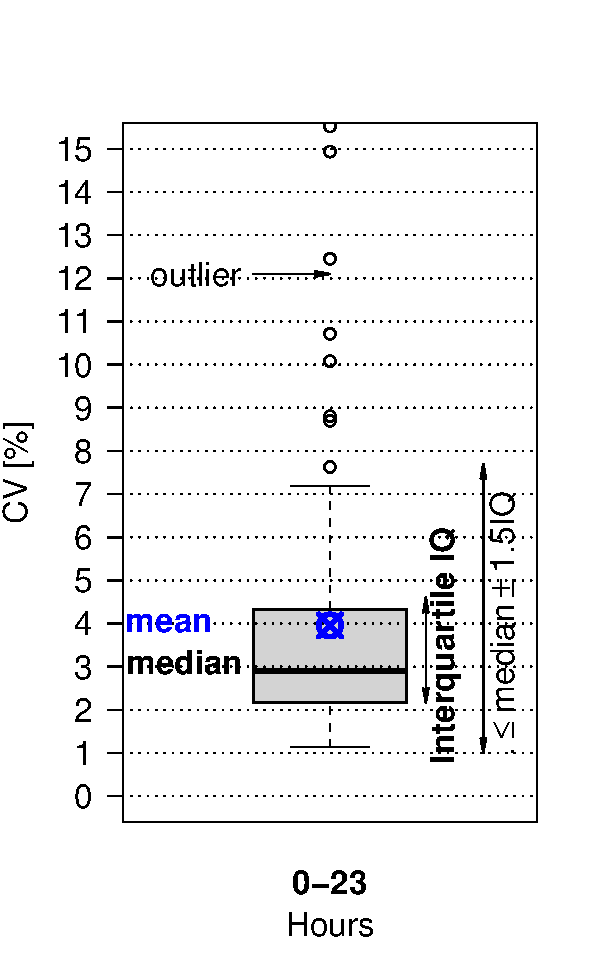
\includegraphics[width=0.3\textwidth]{understanding/figures/var/linkVolumesInterAWTV200.pdf}}%
	%{\label{fig:linkVolumesInterAWTV200}}%
  %{}%
  %\createsubfigure%
  %{Simulated Hourly Volumes (Hour 17-18), Inter-run Variability}%
	%{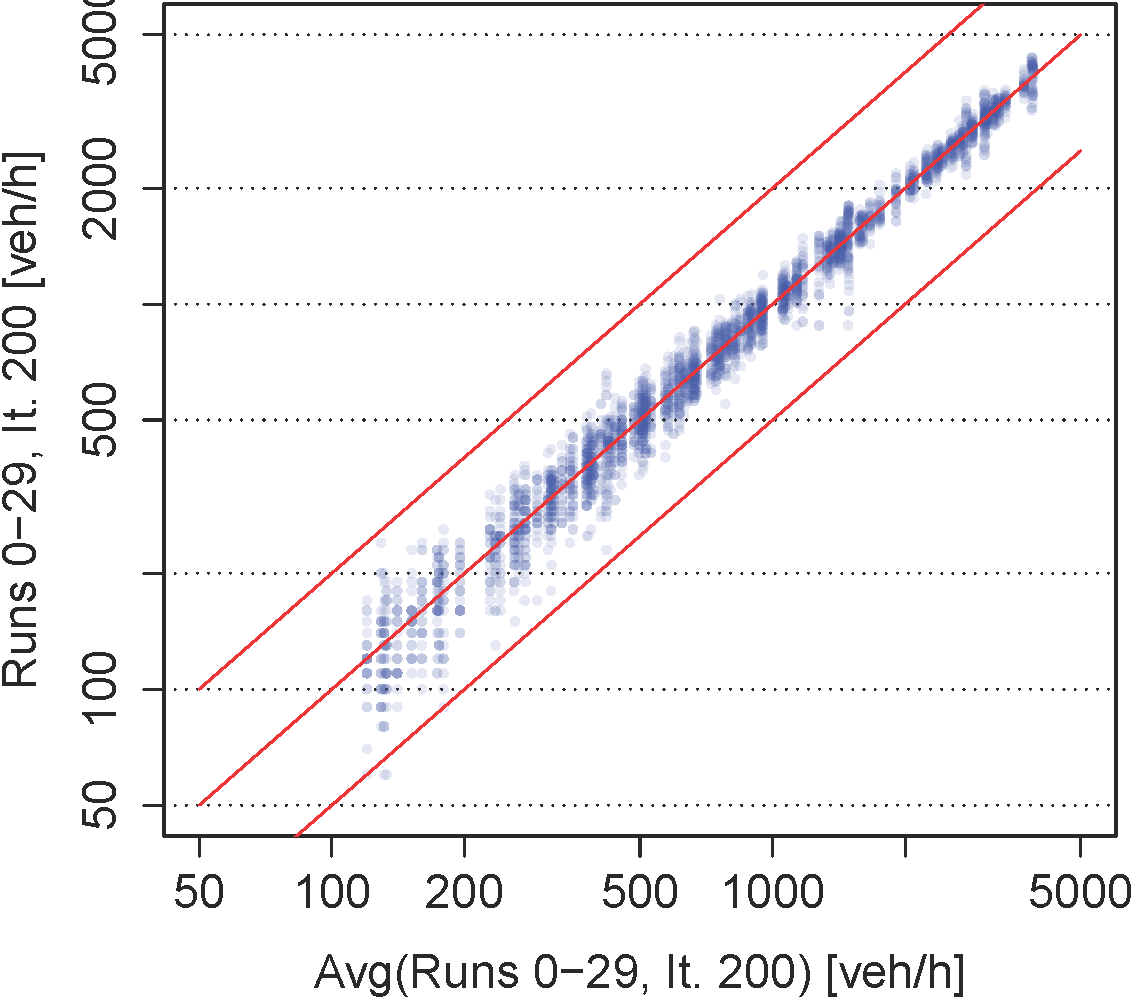
\includegraphics[width=0.49\textwidth]{understanding/figures/var/linkVolumesHour17-18InterScatter.png}}%
	%{\label{fig:linkVolumesHour17-18InterScatter}}%
  %{}%
	%\createsubfigure%
  %{Simulated Hourly Volumes: Inter-run Variability, Runs 0-29, Iteration 200}%
	%{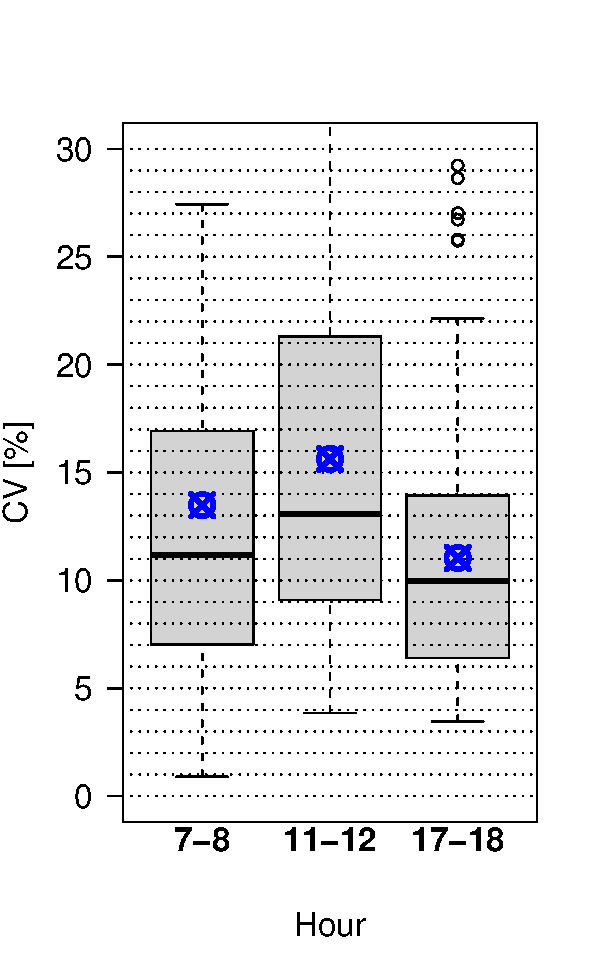
\includegraphics[width=0.3\textwidth]{understanding/figures/var/linkVolumesInter200.pdf}}%
	%{\label{fig:linkVolumesInter200}}%
  %{}%
%}%
%{} 
%
%\vfill\eject
% ##################################################################################################################
% Local Variables:
% mode: latex
% mode: reftex
% mode: visual-line
% TeX-master: "main"
% comment-padding: 1
% fill-column: 9999
% End: 
